%% For double-blind review submission
%\documentclass[sigplan,review,anonymous]{acmart}
%% For single-blind review submission
%\documentclass[sigplan,review]{acmart}
%% For proofreading
% \documentclass[sigplan,authordraft]{acmart}
%% For final camera-ready submission
\documentclass[sigplan]{acmart}
%% For booklet
% \documentclass[acmsmall]{acmart}

% !TEX root=../main.tex


%% Basics %%%%%%%%%%%%%%%%%%%%%%%%%%%%%%%%%%%%%%%%%%%%%%%%%%%%%%%%%%%%%%%%%%%%%%

%% Fixes %%

\usepackage{underscore}


%% Fonts %%

\usepackage[utf8]{inputenc}
% \usepackage[T1]{fontenc}
%%NOTE: T1 doesn't have the `Th` and `Qu` ligatures :-(
\usepackage[OT1]{fontenc}

\usepackage{stmaryrd}

% \usepackage{tgpagella}
% \usepackage{lucidabr}

\usepackage{libertine}
\usepackage[varqu]{zi4}
\usepackage[libertine]{newtxmath}


%% Programming %%

\usepackage{xargs}
\usepackage{ifthen}


%% Layout %%

% \usepackage{microtype}
\usepackage{xspace}


%% Additions %%%%%%%%%%%%%%%%%%%%%%%%%%%%%%%%%%%%%%%%%%%%%%%%%%%%%%%%%%%%%%%%%%%

%% Textual %%

\usepackage{paralist}
\usepackage{quoting}


%% Maths %%

\usepackage{amsmath}
\usepackage{mathpartir}


%% Graphics %%

\usepackage{graphicx}
\usepackage{xcolor}
\usepackage{dblfloatfix}
\usepackage[export]{adjustbox}


%% Tabulations %%

\usepackage{booktabs}
\usepackage{array}


%% Listings %%

\usepackage[final]{listings}


%% References & Bibliography %%

\usepackage{cleveref}
\usepackage{natbib}
% \usepackage[natbibapa,nodoi]{apacite}

% !TEX root=../main.tex


%% Fixes %%

\frenchspacing

%% NOTE: uses the same lengths as in `tufte-common.def` and `article.cls`...
\setlength{\bigskipamount}   {3.25ex plus .2ex} %% ...before (sub)section
\setlength{\medskipamount}   {2.3ex  plus .2ex} %% ...after section
\setlength{\smallskipamount} {1.5ex  plus .2ex} %% ...after subsection


%% Numbering %%

% \setcounter{secnumdepth}{2}


%% Compact lists %%
%% NOTE: requires `paralist`

\setlength{\pltopsep}{\smallskipamount}
\setlength{\plpartopsep}{\parskip}
\setlength{\plitemsep}{\parskip}
\setlength{\plparsep}{\parskip}

% !TEX root=../main.tex


\input macros/auxiliaries


%% Fixes %%%%%%%%%%%%%%%%%%%%%%%%%%%%%%%%%%%%%%%%%%%%%%%%%%%%%%%%%%%%%%%%%%%%%%%

\let\texttilde\textasciitilde


%% Text %%%%%%%%%%%%%%%%%%%%%%%%%%%%%%%%%%%%%%%%%%%%%%%%%%%%%%%%%%%%%%%%%%%%%%%%

\providemacro{marginnote}
  {\marginpar}
\providemacro{smallcaps}
  {\textsc}
\providemacro{marginwidth}
  {\marginparwidth}

\newmacro{alert}[1]
  {\textbf{#1}}
\newmacro{divert}[1]
  {\textcolor{gray}{#1}}
\newmacro{enquote}[1]
  {``#1''}
\newmacro{fixme}[1]
  {\colorbox{yellow}{#1}\marginnote{\colorbox{yellow}{$\star$}}}
\newmacro{todo}[1]
  {\textcolor{red}{$\star$}\marginnote{\textcolor{red}{#1}}}
\newmacro{type}[1]
  {\texttt{#1}}

\newenvironment{fadeout}
  {\color{gray}}
  {}
\newenvironment{emphasize}
  {\begin{quote}\itshape}
  {\end{quote}}
\newenvironment{margintext}[1]
  {\begin{marginfigure}
     \subsection*{#1}}
  {\end{marginfigure}}


%% Lists %%
%% NOTE: requires `paralist`

%% Use compact lists by default
\renewenvironment{itemize}
  {\begin{compactitem}}
  {\end{compactitem}}
\renewenvironment{enumerate}
  {\begin{compactenum}}
  {\end{compactenum}}
\renewenvironment{description}
  {\begin{compactdesc}}
  {\end{compactdesc}}
%% Define starred versions as in-paragraph-lists
\newenvironment{itemize*}
  {\begin{inparaitem}}
  {\end{inparaitem}}
\newenvironment{enumerate*}[1][1=(i)]
  {\begin{inparaenum}[#1]}
  {\end{inparaenum}}
\newenvironment{description*}
  {\begin{inparadesc}}
  {\end{inparadesc}}


%% Quotations %%
%% NOTE: requires `quoting`

\let\quote\quoting
\let\endquote\endquoting
\renewenvironment{quotation}
  {\ClassError{Please use the `quote` environment instead of `quotation`}}


%% Column types %%
%% NOTE: requires `array`

\newcolumntype{L}{>{$}l<{$}}
\newcolumntype{C}{>{$}c<{$}}
\newcolumntype{R}{>{$}r<{$}}
\newcolumntype{T}{>{\ttfamily}l}
\newcolumntype{S}{>{\sffamily}l}


%% References %%
%% NOTE: requires `cleveref`

\let\autoref\cref
\let\Autoref\Cref
\let\autopageref\cpageref


%% Citations %%
%% NOTE: requires `natbib`

\let\cite\citep
\let\Cite\Citep
\let\textcite\citet
\let\Textcite\Citet


%% Blocks and Boxes %%

\newenvironment{block}
  {\begin{center}}
  {\end{center}}
% \newenvironment{box}
%   {\begin{mdframed}}
%   {\end{mdframed}}


%% Logos %%

%% \newlogo[.name.]{.text.}
\newmacro{newlogo}[2][1]
  {\ifthenelse{\isempty{#1}}
     {\newlogoaux{#2}{\smallcaps{\lowercase{#2}}}}
     {\newlogoaux{#1}{#2}}}
\newmacro{newlogoaux}[2]
  {\newmacro{#1}{#2\xspace}}


%% Languages %%%%%%%%%%%%%%%%%%%%%%%%%%%%%%%%%%%%%%%%%%%%%%%%%%%%%%%%%%%%%%%%%%%

%%NOTE: `\mathrel` gives a single space width between keywords but removes it after another relational operator.
%%      `\mathop`  gives just a small skip, but doesn't has above bug.
\newmacro{newoperator}[1]
  {\newmathcommand{#1}[op]}
\newmacro{newkeyword}[2][1]
  %%FIXME: this is to complicated: {\newoperator{\ifthenelse{\isempty{#1}}{#2}{#1}}{\text{\sffamily\bfseries #2}}}
  {\ifthenelse{\isempty{#1}}
    {\newoperator{#2}{\text{\normalfont\sffamily\bfseries #2}}}
    {\newoperator{#1}{\text{\normalfont\sffamily\bfseries #2}}}}
\newmacro{newvalue}[2][1]
  {\ifthenelse{\isempty{#1}}
    {\newoperator{#2}{\text{\normalfont\sffamily #2}}}
    {\newoperator{#1}{\text{\normalfont\sffamily #2}}}}
\newmacro{newtype}[2][1]
  {\ifthenelse{\isempty{#1}}
    {\newoperator{#2}{\text{\normalfont\sffamily\scshape #2}}}
    {\newoperator{#1}{\text{\normalfont\sffamily\scshape #2}}}}


%% Math %%%%%%%%%%%%%%%%%%%%%%%%%%%%%%%%%%%%%%%%%%%%%%%%%%%%%%%%%%%%%%%%%%%%%%%%

%% Symbols %%

%% NOTE: change this to \emptyset when using a font that includes a nice standard emptyset
\let\nothing\varnothing


%% Braces %%

\let\<\langle
\let\>\rangle

\newmathcommand{llbrace}[open] {\{\!|}
\newmathcommand{rrbrace}[close]{|\!\}}

\newmacro{set}[1]
  {\ensuremath{\{#1\}}}
\newmacro{tuple}[1]
  {\ensuremath{\<#1\>}}


%% Operators %%

\let\lt<
\let\gt>
\let\To\Rightarrow

\newmathcommand{pp}[bin]
  {+\!\!+}
\newmathcommand{Mid}
  {\;\mid\;}


%% Shortcuts %%

\newmathcommand{powerset}[cal]{P}

\newmathcommand{n}{\underline{n}}

\newmathcommand{NN}  [bb]{N}
\newmathcommand{ZZ}  [bb]{Z}
\newmathcommand{EE}  [bb]{E}
\newmathcommand{OO}  [bb]{O}
\newmathcommand{QQ}  [bb]{A}
\newmathcommand{RR}  [bb]{R}
\newmathcommand{CC}  [bb]{C}
\newmathcommand{HH}  [bb]{H}

\newmathcommand{LL}  [bb]{L}
\newmathcommand{UU}  [bb]{U}
\newmathcommand{BB}  [bb]{B}
\renewmathcommand{SS}[bb]{S}

\let\to\rightarrow
\let\implies\Rightarrow
\let\infers\vdash


%% Hints and local definitions %%

\newmacro{hint}[1]
  {\quad\text{\{ #1 \}}}

\newmathcommand{when}[op]
  {\mathbf{when}}
\newmathcommand{where}[op]
  {\mathbf{where}}
\renewmathcommand{and}[op]
  {\mathbf{and}}
\newmathcommand{otherwise}[op]
  {\mathbf{otherwise}}
\newmathcommand{impossible}[op]
  {\mathrm{impossible}}


%% Environments %%

\let\group\begingroup

\newenvironment*{marginequation}[1][1=0pt]
  {\begin{marginfigure}[#1]\equation}
  {\endequation\end{marginfigure}}

\newenvironment*{marginequation*}[1][1=0pt]
  {\begin{marginfigure}[#1]\equation\nonumber}
  {\endequation\end{marginfigure}}

\newenvironment*{grammar}
  %%NOTE: the `@{}` suppreses `\tabcolsep` before the first column
  {\begin{block}\begin{tabular}{@{}rRCLl}}
  {\end{tabular}\end{block}}
\newenvironment*{grammar*}
  %%NOTE: the `@{}` suppreses `\tabcolsep` before the first column
  {\begin{block}\begin{tabular}{@{}RLl}}
  {\end{tabular}\end{block}}



%% Theorems %%


\theoremstyle{acmplain}

\newtheorem{theorem}{Theorem}[section]
\newtheorem{conjecture}[theorem]{Conjecture}
\newtheorem{proposition}[theorem]{Proposition}
\newtheorem{lemma}[theorem]{Lemma}
\newtheorem{corollary}[theorem]{Corollary}


\theoremstyle{acmdefinition}

\newtheorem{example}[theorem]{Example}
\newtheorem{definition}[theorem]{Definition}

% !TEX root=../main.tex


%% Styles %%%%%%%%%%%%%%%%%%%%%%%%%%%%%%%%%%%%%%%%%%%%%%%%%%%%%%%%%%%%%%%%%%%%%%

\lstdefinestyle{natural}
  {columns=fullflexible
  ,gobble=2
  ,breaklines=true
  ,breakatwhitespace=true
  ,literate=
    %{.}{{$\cdot$}}1
    %{.}{{\ }}1
    {<<}{{$\<$}}1
    {>>}{{$\>$}}1
    {->}{{$\to$\ }}2
    % {--}{{--}}1
    %{_}{{\ }}1
    %{\ "}{{\ \textquotedblleft}}2
    %{"\ }{{\textquotedblright\ }}2
  ,basicstyle={\sffamily}
  ,keywordstyle=[1]{\bfseries}
  ,keywordstyle=[2]{\scshape}
  ,keywordstyle=[3]{}
  %,commentstyle={\itshape}
  %,identifierstyle={\itshape}
  ,emphstyle={\itshape}
  %,stringstyle={\rmfamily}
  ,showstringspaces=false
  ,texcl=true
  ,mathescape=true
  %,escapechar=\$
  %,escapeinside={\{\}}
  ,xleftmargin=1\parindent
  }

\lstdefinestyle{flexible}
  {columns=flexible
  ,gobble=2
  ,fontadjust=true
  ,basicstyle={\ttfamily\small}
  ,commentstyle={\itshape}
  ,keywordstyle={\bfseries}
  %,identifierstyle={\itshape}
  %,stringstyle={\ttfamily}
  ,emphstyle={\itshape}
  ,showstringspaces=false
  ,texcl=true
  ,mathescape=true
  %,escapechar=\$
  %,escapeinside={\{\}}
  ,xleftmargin=1\parindent
  }

\lstdefinestyle{literate}
  {style=natural
  ,literate=
    {\\}{{$\lambda$}}1
    {\\\$}{{\$}}1 %NOTE: otherwise eaten by `\`, NOTE: prevents \$ to be parsed as math escape
    {\\/}{{$\vee$}}1
    {/\\}{{$\wedge$}}1
    {A.}{{$\forall$}}1
    {E.}{{$\exist$}}1
    {->}{{$\rightarrow$ }}1
    {<-}{{$\leftarrow$}}1
    {==}{{$\equiv$\ }}1
    {/=}{{$\nequiv$\ }}1
    {<=}{{$\leq$}}1
    {>=}{{$\geq$}}1
    {>>=}{{>>=}}3 %NOTE: otherwise eaten by `>=`
    {\{|}{{$\{\!|\!$}}1
    {|\}}{{$\!|\!\}$}}1
    {\{|*|\}}{{$\{\!|\!\!\star\!\!|\!\}$}}3
  }


%% Definitions %%%%%%%%%%%%%%%%%%%%%%%%%%%%%%%%%%%%%%%%%%%%%%%%%%%%%%%%%%%%%%%%%

%% Tasks %%

\lstdefinelanguage{tasks}
  {sensitive=true
  ,morekeywords=[1]{let,in,if,then,else,case,of,ref,type}
  ,morekeywords=[2]{Bool,Int,String,Store,List,Passenger,Seat,Booking}
  ,morestring=[b]"
  ,morecomment=[l]--
  ,morecomment=[n]{\{-}{-\}}
  }[keywords,strings,comments]
\lstdefinestyle{tasks}
  {style=natural
  ,literate=
    {\\}{{$\lambda$}}1
    {<<}{{$\<$}}1
    {>>}{{$\>$}}1
    {==}{{$\equiv$\ }}1
    {/=}{{$\nequiv$\ }}1
    {<=}{{$\leq$\ }}1
    {>=}{{$\geq$\ }}1
    {*}{{$\times$\ }}1
    {\\/}{{$\vee$\ }}1
    {/\\}{{$\wedge$\ }}1
    {>>=}{{$\Then$\ }}1
    {>>?}{{$\Next$\ }}1
    {<&>}{{$\And$\ }}1
    {<|>}{{$\Or$\ }}1
    {<?>}{{$\Xor$\ }}1
    {edit}{{$\Edit$}}1
    {enter}{{$\Enter$}}1
    {update}{{$\Update$}}1
    {fail}{{$\Fail$\ }}1
  }

\lstnewenvironment{TASK}[1][]
  {\lstset{language=tasks,style=tasks,#1}}
  {}
\newmacro{TS}[1][1]
  {\lstinline[language=tasks,style=tasks,#1]}
\newmacro{includeTASK}[2][]
  {\lstinputlisting[language=tasks,style=tasks,#1]{#2}}


%% Flows %%

\lstdefinelanguage{flows}
  {sensitive=true
  ,morekeywords=[1]{module,where,define,using,as,yielding,share,holding,with,do,for,fork,then,when,next,done,on,and,or,not,readonly,writeonly,readwrite}
  ,morekeywords=[2]{Bool,Int,String,Shared,List, Date,Document,Photo, Citizen,Company,Declaration}
  ,morekeywords=[3]{True,False,Just,Nothing,List}
  ,morestring=[b]"
  ,morecomment=[l]--
  ,morecomment=[n]{\{-}{-\}}
  }[keywords,strings,comments]

% \lstMakeShortInline[language=flows,style=natural] | % |
\lstnewenvironment{FLOW}[1][]
  {\lstset{language=flows,style=natural,#1}}
  {}
\newmacro{FL}[1][1]
  {\lstinline[language=flows,style=natural,#1]}
\newmacro{includeFLOW}[2][]
  {\lstinputlisting[language=flows,style=natural,#1]{#2}}


%% Clean %%

\lstdefinelanguage{clean}
  {sensitive=true
  %,alsoletter={ABCDEFGHIJKLMNOPQRSTUVWXYZabcdefghijklmnopqrstuvwxyz_`}
  %,alsoletter={~!@\#$\%^\&*-+=?<>:|\\} %$
  ,morekeywords={from,definition,implementation,import,module,system,code,inline,if,case,of,let,let!,in,where,with,class,instance,generic,derive,dynamic,infix,infixl,infixr}
  ,morestring=[b]"
  ,morestring=[b]'
  ,morecomment=[l]//
  ,morecomment=[n]{/*}{*/}
  }[keywords,strings,comments]

\lstnewenvironment{CLEAN}[1][]
  {\lstset{language=clean,style=flexible,#1}}
  {}
\newmacro{CL}[1][1]
  {\lstinline[language=clean,style=flexible,#1]}
\newmacro{includeCLEAN}[2][1]
  {\lstinputlisting[language=clean,style=flexible,#1]{#2}}

% !TEX root=../main.tex

\newcommand*{\GUI}
  {\smallcaps{gui}}
\newcommand*{\ITASKS}
  {\smallcaps{iTasks}}

% !TEX root=../main.tex


\newlogo{Lang}


%% Host language %%%%%%%%%%%%%%%%%%%%%%%%%%%%%%%%%%%%%%%%%%%%%%%%%%%%%%%%%%%%%%%

\newkeyword[IF]  {if}
\newkeyword[THEN]{then}
\newkeyword[ELSE]{else}

\newkeyword[Ref] {ref}

\newmacro{If}[3]
  {\IF #1 \THEN #2 \ELSE #3}


%% Values %%

\newvalue{True}
\newvalue{False}

\newmacro{str}[1]
  {\text{``#1''}}


%% Types %%

\newtype{Unit}
\newtype{Bool}
\newtype{Nat}
\newtype{Int}
\newtype{String}
\newtype[Reference]{Ref}
\newtype{Task}

\newtype{Euro}


%% Object language %%%%%%%%%%%%%%%%%%%%%%%%%%%%%%%%%%%%%%%%%%%%%%%%%%%%%%%%%%%%%

\let\And\relax
\newoperator{Then}  {\blacktriangleright}
\newoperator{ExThen}{\vartriangleright}
\newoperator{And}   {\Join}
\newoperator{Or}    {\blacklozenge}
\newoperator{ExOr}  {\;\lozenge\;}
\newoperator{Edit}  {\square}
\newoperator{Fill}  {\boxtimes}
\newoperator{Change}{\blacksquare}
\newoperator{Fail}  {\lightning}

\newoperator{AndOr} {\DEPRECATED}


%% Events %%

\newvalue[Left]   {L}
\newvalue[Right]  {R}

\newvalue[Clear]  {C}
\newvalue[Next]   {N}
\newvalue[Pick]   {P}

\newvalue[First]  {F}
\newvalue[Second] {S}
\newvalue[Other]  {S}


%% Semantic functions %%%%%%%%%%%%%%%%%%%%%%%%%%%%%%%%%%%%%%%%%%%%%%%%%%%%%%%%%%

\newmathcommand{evaluate}[rel]
  {\Downarrow}
\newmathcommand{normalise}[rel]
  % {\;\rightarrow\!\shortmid\;}
  {\downarrow}
\newmacro{handle}[1]
  {\mathrel{\;\xrightarrow{\;#1\;}\;}}

\newmathcommand{Observe}[cal]
  {O}


%% Depricated %%%%%%%%%%%%%%%%%%%%%%%%%%%%%%%%%%%%%%%%%%%%%%%%%%%%%%%%%%%%%%%%%%

\newvalue[Execute] {<depricated>}

% !TEX root=main.tex


%% Helpers %%%%%%%%%%%%%%%%%%%%%%%%%%%%%%%%%%%%%%%%%%%%%%%%%%%%%%%%%%%%%%%%%%%%%

\newmacro{newrule}[4][2]
  {\newmacro{#1}{\inferrule*[lab={#1},right={$#2$}]
    {#3}
    {#4}}}
\newmacro{userule}
  {\usemacro}
\newmacro{refrule}[1]
  {\ifthenelse{\isundefined{#1}}
    {\GenericError{}{Rule `#1` is not defined}{}{}}
    {\textsc{#1}}}


\newif\ifstateful
\statefulfalse
\newmacro{st}[1]
  {\ifstateful{, #1}\else{}\fi}



%% Typing %%%%%%%%%%%%%%%%%%%%%%%%%%%%%%%%%%%%%%%%%%%%%%%%%%%%%%%%%%%%%%%%%%%%%%


\newmacro{RelationT}
  {\Gamma\st{\Sigma} \infers e : \tau}


\newrule{T-Edit}
  {\Gamma\st{\Sigma} \infers e : \beta}
  {\Gamma\st{\Sigma} \infers \Edit e : \Task \beta}


\newrule{T-Fill}
  {\ }
  {\Gamma\st{\Sigma} \infers \Fill \beta : \Task \beta}


\newrule{T-Change}
  {\Gamma, \Sigma \infers e : \beta}
  {\Gamma, \Sigma \infers \Change e : \Task \beta}


\newrule{T-Fail}
  { }
  {\Gamma\st{\Sigma} \infers \Fail : \forall\alpha. \Task \alpha}


\newrule{T-Next}
  {\Gamma\st{\Sigma} \infers e_1 : \Task \tau_1 \\
   \Gamma\st{\Sigma} \infers e_2 : \tau_1 \to \Task \tau_2}
  {\Gamma\st{\Sigma} \infers e_1 \Next e_2 : \Task \tau_2}


\newrule{T-Then}
  {\Gamma\st{\Sigma} \infers e_1 : \Task \tau_1 \\
   \Gamma\st{\Sigma} \infers e_2 : \tau_1 \to \Task \tau_2}
  {\Gamma\st{\Sigma} \infers e_1 \Then e_2 : \Task \tau_2}


\newrule{T-All}
  {\Gamma\st{\Sigma} \infers e_1 : \Task \tau_1 \\
   \Gamma\st{\Sigma} \infers e_2 : \Task \tau_2}
  {\Gamma\st{\Sigma} \infers e_1 \And e_2 : \Task\,(\tau_1 \times \tau_2)}


\newrule{T-One}
  {\Gamma\st{\Sigma} \infers e_1 : \Task \tau \\
   \Gamma\st{\Sigma} \infers e_2 : \Task \tau }
  {\Gamma\st{\Sigma} \infers e_1 \Xor e_2 : \Task \tau}



%% Evaluation %%%%%%%%%%%%%%%%%%%%%%%%%%%%%%%%%%%%%%%%%%%%%%%%%%%%%%%%%%%%%%%%%%


\newmacro{RelationV}
  {e \evaluate v}


\newrule{E-Edit}
  {e \evaluate v}
  {\Edit e \evaluate \Edit v}


\newrule{E-Fill}
  {\ }
  {\Fill \beta \evaluate \Fill \beta}


\newrule{E-Fail}
  { }
  {\Fail \evaluate \Fail}


\newrule{E-Then}
  {e_1 \evaluate t_1}
  {e_1 \Then e_2 \evaluate t_1 \Then e_2}



%% Normalisation %%%%%%%%%%%%%%%%%%%%%%%%%%%%%%%%%%%%%%%%%%%%%%%%%%%%%%%%%%%%%%%


\newmacro{RelationN}
  {t\st{s} \normalise t'\st{s'}}


\newrule{N-Edit}
  { }
  {\Edit v \normalise \Edit v}


\newrule{N-Fill}
  { }
  {\Fill \beta \normalise \Fill \beta}


\newrule{N-Fail}
  { }
  {\Fail \normalise \Fail}


\newrule{N-ThenStay}[\Value(t_1') = \bot]
  {t_1\st{s} \normalise t_1'\st{s'}}
  {t_1 \Then e_2\st{s} \normalise t_1' \Then e_2\st{s'}}


\newrule{N-ThenFail}[\Value(t_1') = v_1 \land \lnot\Succeeding(t_2)]
  {t_1\st{s} \normalise t_1'\st{s'} \\
   e_2\ v_1 \evaluate t_2}
  {t_1 \Then e_2\st{s} \normalise t_1' \Then e_2\st{s'}}


\newrule{N-ThenCont}[\Value(t_1') = v_1 \land \Succeeding(t_2)]
  {t_1\st{s} \normalise t_1'\st{s'} \\
   e_2\ v_1 \evaluate t_2  \\
   t_2\st{s'} \normalise t_2'\st{s''}}
  {t_1 \Then e_2\st{s} \normalise t_2'\st{s''}}


%%%%

\newrule{N-Interact}
  { }
  {u\st{s} \normalise u\st{s}}

% \newrule{N-Change}
%   { }
%   {\Change l\st{s} \normalise \Change l\st{s}}

% \newrule{N-Next}[t_1' = \Edit v]
%   {t_1\st{s} \normalise t_1'\st{s'}   \\
%    e\ v \evaluate t_2       \\
%    t_2\st{s'} \normalise t_2'\st{s''} }
%   {t_1 \Next e\st{s} \normalise t_2'\st{s''}}

\newrule{N-All}[t_1' = \Edit v_1 \land t_2' = \Edit v_2]
  {t_1\st{s}  \normalise t_1'\st{s'}  \\
   t_2\st{s'} \normalise t_2'\st{s''} }
  {t_1 \And t_2\st{s} \normalise \Edit \{v_1, v_2\}\st{s}}

\newrule{N-NextEval}
  {e_1\st{s} \normalise u_1\st{s'}}
  {e_1 \Next e_2\st{s} \normalise u_1 \Next e_2\st{s'}}

\newrule{N-AndEval}
  {e_1\st{s}  \normalise u_1\st{s'}  \\
   e_2\st{s'} \normalise u_2\st{s''} }
  {e_1 \And e_2\st{s} \normalise u_1 \And u_2\st{s}}

% \newrule{N-OrEval}[t_1' \neq \Edit v_1 \land t_2' \neq \Edit v_2]
%   {t_1\st{s}  \normalise t_1'\st{s'}  \\
%    t_2\st{s'} \normalise t_2'\st{s''} }
%   {t_1 \Xor t_2\st{s} \normalise t_1' \Xor t_2'\st{s}}



%% Handling %%


\newmacro{RelationH}
  {t\st{s} \handle{h} t'\st{s'}}


\newrule{H-Change}[v, v' : \beta]
  { }
  {\Edit v\st{s} \handle{v'} \Edit v'\st{s}}


\newrule{H-Clear}[v : \beta]
  { }
  {\Edit v\st{s} \handle{\Clear} \Fill \beta\st{s}}


\newrule{H-Fill}[v' : \beta]
  { }
  {\Fill \beta\st{s} \handle{v'} \Edit v'\st{s}}


\newrule{H-Fail}
  { }
  {\Fail\st{s} \handle{h} \Fail\st{s}}


%%%%


\newrule{H-Store}[\Sigma(l), v' : \tau]
  { }
{\Change l, s \handle{v'} \Change l, [l \mapsto v']s}

\newrule{H-Stay'}[\Value(t_1) = \bot]
  {\ }
  {t_1 \Next e\st{s} \handle{\Next} t_1 \Next e\st{s}}

\newrule{H-Next'}[\Value(t_1) = v]
  {e\ v \evaluate t_2    \\
   t_2\st{s} \normalise t_2'\st{s'} }
  {t_1 \Next e\st{s} \handle{\Next} t_2'\st{s'}}

\newrule{H-Stay}[\Value(t_1) = \bot]
  {\ }
  {t_1 \Then e\st{s} \handle{\Execute \pi} t_1 \Then e\st{s}}

\newrule{H-Fail'}[\Value(t_1) = v \land t_2 = \Fail]
  {e\ v \evaluate t_2    \\
   t_2\st{s} \handle{\Pick \pi} t_2'\st{s'} }
  {t_1 \Then e\st{s} \handle{\Execute \pi} t_1 \Then e\st{s}}

\newrule{H-Next}[\Value(t_1) = v \land t_2 \neq \Fail]
  {e\ v \evaluate t_2    \\
   t_2\st{s} \handle{\Pick \pi} t_2'\st{s'} }
  {t_1 \Then e\st{s} \handle{\Execute \pi} t_2'\st{s'}}

\newrule{H-PassS}
  {t_1\st{s} \handle{h} t_1'\st{s'}}
  {t_1 \Next e\st{s} \handle{h} t_1' \Next e\st{s'}}

\newrule{H-Pass}[h \neq \Execute \pi]
  {t_1\st{s} \handle{h} t_1'\st{s'}       \\
   t_1' \Then e\st{s'} \normalise t_2\st{s''} }
  {t_1 \Then e\st{s} \handle{h} t_2\st{s''}}

\newrule{H-First}[t_1 \neq \Fail]
  {\ }
  {t_1 \Xor t_2\st{s} \handle{\Pick \First} t_1\st{s}}

\newrule{H-Second}[t_2 \neq \Fail]
  {\ }
  {t_1 \Xor t_2\st{s} \handle{\Pick \Second} t_2\st{s}}

\newrule{H-Other}[t_2 \neq \Fail]
  {t_2\st{s} \handle{\Pick \pi} t_2'\st{s'}}
  {t_1 \Xor t_2\st{s} \handle{\Pick \Other \pi} t_2'\st{s'}}

\newrule{H-Left}
  {t_1\st{s} \handle{h} t_1'\st{s'} }
  {t_1 \AndOr t_2\st{s} \handle{\Left h} t_1' \AndOr t_2\st{s'}}

\newrule{H-Right}
  {t_2\st{s} \handle{h} t_2'\st{s'} }
  {t_1\st{s} \AndOr t_2 \handle{\Right h} t_1 \AndOr t_2'\st{s'}}

\newrule{H-Fallback}
  { }
  {t\st{s} \handle{h} t\st{s}}

% !TEX root=pldi2019.tex


%% Language %%%%%%%%%%%%%%%%%%%%%%%%%%%%%%%%%%%%%%%%%%%%%%%%%%%%%%%%%%%%%%%%%%%%

\newmacro{G-Language}{
  \begin{grammar}
    Expressions
      & e    &::= & \lambda x:\tau.\ e   & – abstraction \\
      &      &\mid& e_1\ e_2             & – application \\
      &      &\mid& x                    & – variable \\
      &      &\mid& c                    & – constant \\
    \addlinespace
      &      &\mid& e_1 \star e_2        & – operation \\
      &      &\mid& \If{e_1}{e_2}{e_3}   & – branch \\
      &      &\mid& \tuple{e_1, e_2}     & – pair \\
      &      &\mid& \unit                & – unit \\
    \addlinespace
      &      &\mid& \Ref e               & – reference \\
      &      &\mid& !e                   & – dereference \\
      &      &\mid& e_1 := e_2           & – assignment \\
      % &      &\mid& e_1; e_2             & – sequence \\
      &      &\mid& l                    & – location \\
    \addlinespace
      &      &\mid& p                    & – pretask \\
    \addlinespace
    Constants
      & c    &::= & B                    & – boolean \\
      &      &\mid& I                    & – integer \\
      &      &\mid& S                    & – string \\
  \end{grammar}
}

\newmacro{G-Pretasks}{
  \begin{grammar}
    Pretasks
      & p    &::= & \Edit e              & – valued editor \\
      &      &\mid& \Enter \beta         & – unvalued editor \\
      &      &\mid& \Update e            & – stored editor \\
    \addlinespace
      &      &\mid& e_1 \Then e_2        & – step \\
      &      &\mid& e_1 \Next e_2        & – user step \\
    \addlinespace
      &      &\mid& e_1 \And e_2         & – composition \\
    \addlinespace
      &      &\mid& e_1 \Or e_2          & – choice \\
      &      &\mid& e_1 \Xor e_2         & – user choice \\
    \addlinespace
      &      &\mid& u \At e              & – appoint \\
      &      &\mid& \Fail                & – fail task \\
  \end{grammar}
}

\newmacro{G-Types}{
  \begin{grammar}
    Types
      & \tau &::= & \tau_1 \to \tau_2    & – function type \\
      &      &\mid& \tau_1 \times \tau_2 & – product type \\
      &      &\mid& \Unit                & – unit type \\
      &      &\mid& \Reference \tau      & – reference type \\
      &      &\mid& \Task \tau           & – task type \\
      &      &\mid& \beta                & – basic type \\
      % &      &\mid& \alpha               & – universal type \\
    Basic types
      &\beta &::= & \Bool                & – boolean type \\
      &      &\mid& \Int                 & – integer type \\
      &      &\mid& \String              & – string type \\
  \end{grammar}
}

\newmacro{G-Values}{
  \begin{grammar}
    Values
      & v    &::= & \lambda x:\tau.\ e        & – abstraction \\
      &      &\mid& \tuple{v_1, v_2}     & – pair value \\
      &      &\mid& \unit                & – unit \\
      &      &\mid& c                    & – constant \\
      &      &\mid& l                    & – location \\
      &      &\mid& t                    & – task \\
    Tasks
      & t    &::= & \Edit v              & – valued editor \\
      &      &\mid& \Enter \beta         & – unvalued editor \\
      &      &\mid& \Update l            & – stored editor \\
      &      &\mid& \Fail                & – fail task \\
      &      &\mid& t_1 \Then e_2        & – step \\
      &      &\mid& t_1 \Next e_2        & – user step \\
      &      &\mid& t_1 \And t_2         & – composition \\
      &      &\mid& t_1 \Or t_2          & – choice \\
      &      &\mid& t_1 \Xor t_2         & – user choice \\
  \end{grammar}
}

\newmacro{G-Inputs}{
  \begin{grammar}
    Inputs
      & i    & ::=& a                    & – action \\
      &      &\mid& \First i             & – pass to first \\
      &      &\mid& \Second i            & – pass to second \\
    Actions
      & a    & ::=& v                    & – change editor to value \\
      &      &\mid& \Empty               & – empty an editor \\
      &      &\mid& \Continue            & – continue with next task \\
      &      &\mid& \Pick                & – pick route \\
    Routes
      & r    & ::=& \Left                & – go left \\
      &      &\mid& \Right               & – go right \\
  \end{grammar}
}

% !TEX root=pldi2019.tex


%% Language %%%%%%%%%%%%%%%%%%%%%%%%%%%%%%%%%%%%%%%%%%%%%%%%%%%%%%%%%%%%%%%%%%%%

\newmacro{O-Value}{
  \begin{function}
    \signature{\Value : \mathrm{Tasks} \times \mathrm{States} \rightharpoonup \mathrm{Values}} \\
    \Value(\Edit v, s)                &=& v \\
    \Value(\Enter \tau, s)            &=& \bot \\
    \Value(\Update l, s)              &=& s(l) \\
    \Value(\Fail, s)                  &=& \bot \\
    \Value(t_1 \Then e_2, s)          &=& \bot \\
    \Value(t_1 \Next e_2, s)          &=& \bot \\
    \Value(t_1 \And t_2, s)           &=& \left\{
      \begin{array}{l@{}l}
        \tuple{v_1, v_2}              & \ \when\ \Value(t_1, s) = v_1 \land \Value(t_2, s) = v_2 \\
        \bot                          & \ \otherwise
      \end{array}
    \right. \\
    \Value(t_1 \Or t_2, s)            &=& \left\{
      \begin{array}{l@{}l}
        v_1                           & \ \when\ \Value(t_1, s) = v_1 \\
        v_2                           & \ \when\ \Value(t_1, s) = \bot \land \Value(t_2, s) = v_2 \\
        \obox{\tuple{v_1, v_2}}{\bot} & \ \otherwise
      \end{array}
    \right. \\
    \Value(t_1 \Xor t_2, s)           &=& \bot \\
    \Value(u \At t, s)                &=& \Value(t,s)
  \end{function}
}

\newmacro{O-Value-Compact}{
  \begin{function}
    \signature{\Value : \mathrm{Tasks} \times \mathrm{States} \rightharpoonup \mathrm{Values}} \\
    \Value(\Edit v, s)                &=& v \\
    \Value(\Enter \tau, s)            &=& \bot \\
    \Value(\Update l, s)              &=& s(l) \\
    \Value(\Fail, s)                  &=& \bot \\
    \Value(t_1 \Then e_2, s)          &=& \bot \\
    \Value(t_1 \Next e_2, s)          &=& \bot \\
    \Value(t_1 \And t_2, s)           &=& \left\{
      \begin{array}{@{}l@{\  }l@{}}
        \tuple{v_1, v_2}              & \when\ \Value(t_1, s) = v_1 \\
                                      & \multicolumn{1}{r@{}}{\mathbf{and\ } \Value(t_2, s) = v_2} \\
        \bot                          & \otherwise
      \end{array}
    \right. \\
    \Value(t_1 \Or t_2, s)            &=& \left\{
      \begin{array}{@{}l@{\  }l@{}}
        v_1                           & \when\ \Value(t_1, s) = v_1 \\
        v_2                           & \when\ \Value(t_1, s) = \bot \\
                                      & \multicolumn{1}{r@{}}{\mathbf{and\ } \Value(t_2, s) = v_2} \\
        \obox{\tuple{v_1, v_2}}{\bot} & \otherwise
      \end{array}
    \right. \\
    \Value(t_1 \Xor t_2, s)           &=& \bot \\
    \Value(u \At t, s)                &=& \Value(t,s)
  \end{function}
}

\newmacro{O-Value-Compact-Old}{
  \begin{function}
    \signature{\Value : \mathrm{Tasks} \times \mathrm{States} \rightharpoonup \mathrm{Values}} \\
    \Value(\Edit v, s)       &=& v \\
    \Value(\Enter \tau, s)   &=& \bot \\
    \Value(\Update l, s)     &=& s(l) \\
    \Value(\Fail, s)         &=& \bot \\
    \Value(t_1 \Then e_2, s) &=& \bot \\
    \Value(t_1 \Next e_2, s) &=& \bot \\
    \Value(t_1 \And t_2, s)  &=& \tuple{v_1, v_2} \\
      \inset{\when\ \Value(t_1, s) = v_1 \land \Value(t_2, s) = v_2} \\
                             &=& \bot \quad \otherwise \\
    \Value(t_1 \Or t_2, s)   &=& v_1 \quad \when\ \Value(t_1, s) = v_1 \\
                             &=& v_2 \\
      \inset{\when\ \Value(t_1, s) = \bot \land \Value(t_2, s) = v_2} \\
                             &=& \bot \quad \otherwise \\
    \Value(t_1 \Xor t_2, s)  &=& \bot \\
    \Value(u \At t, s)       &=& \Value(t,s)
  \end{function}
}


\newmacro{O-Inputs}{
  \begin{function}
    \signature{\Inputs : \mathrm{Tasks} \times \mathrm{States} \to \powerset(\mathrm{Inputs})} \\
    \Inputs(\Edit v,s)             &=& \set{v':\tau, \Empty}                       \quad\where\ \Edit v : \Task\tau \\
    \Inputs(\Enter \tau,s)         &=& \set{v':\tau} \\
    \Inputs(\Update l,s)           &=& \obox{\set{v':\tau, \Empty}}{\set{v':\tau}} \quad\where\ \Update l : \Task\tau \\
    \Inputs(\Fail,s)               &=& \nothing \\
    \Inputs(t_1 \Then e_2,s)       &=& \Inputs(t_1,s) \\
    \Inputs(t_1 \Next e_2,s)       &=& \Inputs(t_1,s) \cup \{\Continue \mid \Value(t_1, s) = v_1 \land \phantom{} \\
                                   & & \quad e_2\ v_1, s \normalise t_2, s' \land \lnot\Failing(t_2, s')\} \\
    \Inputs(t_1 \And t_2,s)        &=& \set{\First\ i \mid i \in \Inputs(t_1,s)} \cup \set{\Second\ i \mid i \in \Inputs(t_2,s)} \\
    \Inputs(t_1 \Or t_2,s)         &=& \set{\First\ i \mid i \in \Inputs(t_1,s)} \cup \set{\Second\ i \mid i \in \Inputs(t_2,s)} \\
    \Inputs(e_1 \Xor e_2,s)        &=& \set{\Pick \obox{\Right}{\Left} \mid e_1, s \normalise t_1, s' \land \lnot\Failing(t_1, s')} \cup \phantom{} \\
                                   & & \set{\Pick \Right \mid e_2, s \normalise t_2, s' \land \lnot\Failing(t_2, s')} \\
    \Inputs(u_1 \At t,s)           &=& \set{u_2 \At i\mid u_2 \At i \in \Inputs(t,s)} \cup \set{u_1 \At i\mid i\in \Inputs(t,s)}
  \end{function}
}

\newmacro{O-Inputs-Compact}{
  \begin{function}
    \signature{\Inputs : \mathrm{Tasks} \times \mathrm{States} \to \powerset(\mathrm{Inputs})} \\
    \Inputs(\Edit v,s)             &=& \set{v':\tau, \Empty}                       \quad\where\ \Edit v : \Task\tau \\
    \Inputs(\Enter \tau,s)         &=& \set{v':\tau} \\
    \Inputs(\Update l,s)           &=& \obox{\set{v':\tau, \Empty}}{\set{v':\tau}} \quad\where\ \Update l : \Task\tau \\
    \Inputs(\Fail,s)               &=& \nothing \\
    \Inputs(t_1 \Then e_2,s)       &=& \Inputs(t_1,s) \\
    \Inputs(t_1 \Next e_2,s)       &=& \Inputs(t_1,s) \cup \{\Continue \mid \Value(t_1, s) = v_1 \land \phantom{} \\
                                   & & \quad e_2\ v_1, s \normalise t_2, s' \land \lnot\Failing(t_2, s')\} \\
    \Inputs(t_1 \And t_2,s)        &=& \set{\First\ i \mid i \in \Inputs(t_1,s)} \\
                                &\cup& \set{\Second\ i \mid i \in \Inputs(t_2,s)} \\
    \Inputs(t_1 \Or t_2,s)         &=& \set{\First\ i \mid i \in \Inputs(t_1,s)} \\
                                &\cup& \set{\Second\ i \mid i \in \Inputs(t_2,s)} \\
    \Inputs(e_1 \Xor e_2,s)        &=& \set{\Pick \obox{\Right}{\Left} \mid e_1, s \normalise t_1, s' \land \lnot\Failing(t_1, s')} \\
                                &\cup& \set{\Pick \Right \mid e_2, s \normalise t_2, s' \land \lnot\Failing(t_2, s')} \\
    \Inputs(u_1 \At t,s)           &=& \set{u_2 \At i\mid u_2 \At i \in \Inputs(t,s)} \\
                                &\cup& \set{u_1 \At i\mid i\in \Inputs(t,s)}
  \end{function}
}


\newmacro{O-Failing}{
  \begin{function}
    \signature{\Failing : \mathrm{Tasks} \times \mathrm{States} \to \mathrm{Booleans}} \\
    \Failing(\Edit v,s)       &=& \False \\
    \Failing(\Enter \tau,s)   &=& \False \\
    \Failing(\Update l,s)     &=& \False \\
    \Failing(\Fail,s)         &=& \True \\
    \Failing(t_1 \Then e_2,s) &=& \Failing(t_1,s) \\
    \Failing(t_1 \Next e_2,s) &=& \Failing(t_1,s) \\
    \Failing(t_1 \And t_2,s)  &=& \Failing(t_1,s) \land \Failing(t_2,s) \\
    \Failing(t_1 \Or t_2,s)   &=& \Failing(t_1,s) \land \Failing(t_2,s) \\
    \Failing(e_1 \Xor e_2,s)  &=& \Failing(t_1,s_1') \land \Failing(t_2,s_2') \\
      % \inset{\where\ e_1,s \normalise t_1,s_1' \mathbf{\ and\ } e_2,s \normalise t_2,s_2'} \\
                              & & \quad\where\ e_1,s \normalise t_1,s_1' \mathbf{\ and\ } e_2,s \normalise t_2,s_2' \\
    \Failing(u \At t,s)       &=& \Failing(t,s)
  \end{function}
}

\newmacro{O-Failing-Compact}{
  \begin{function}
    \signature{\Failing : \mathrm{Tasks} \times \mathrm{States} \to \mathrm{Booleans}} \\
    \Failing(\Edit v,s)       &=& \False \\
    \Failing(\Enter \tau,s)   &=& \False \\
    \Failing(\Update l,s)     &=& \False \\
    \Failing(\Fail,s)         &=& \True \\
    \Failing(t_1 \Then e_2,s) &=& \Failing(t_1,s) \\
    \Failing(t_1 \Next e_2,s) &=& \Failing(t_1,s) \\
    \Failing(t_1 \And t_2,s)  &=& \Failing(t_1,s) \land \Failing(t_2,s) \\
    \Failing(t_1 \Or t_2,s)   &=& \Failing(t_1,s) \land \Failing(t_2,s) \\
    \Failing(e_1 \Xor e_2,s)  &=& \Failing(t_1,s_1') \land \Failing(t_2,s_2') \\
                              \multicolumn{3}{R@{}}{\where\ e_1,s \normalise t_1,s_1'} \\
                              \multicolumn{3}{R@{}}{\mathbf{and\ } e_2,s \normalise t_2,s_2'} \\
    \Failing(u \At t,s)       &=& \Failing(t,s) \\
                              & & \\
                              & & \\
                              & & \\
  \end{function}
}


\newmacro{O-Watching}{
  \begin{function}
    \signature{\Watching : \mathrm{Tasks} \to \powerset(\mathrm{Locations})} \\
    \Watching(\Edit v)       &=& \nothing \\
    \Watching(\Enter \tau)   &=& \nothing \\
    \Watching(\Update l)     &=& \set{l} \\
    \Watching(\Fail)         &=& \nothing\\
    \Watching(t_1 \Then e_2) &=& \Watching(t_1) \\
    \Watching(t_1 \Next e_2) &=& \Watching(t_1) \\
    \Watching(t_1 \And t_2)  &=& \Watching(t_1) \cup \Watching(t_2) \\
    \Watching(t_1 \Or t_2)   &=& \Watching(t_1) \cup \Watching(t_2) \\
    \Watching(e_1 \Xor e_2)  &=& \nothing \\
    \Watching(u \At t)       &=& \Watching(t)
  \end{function}
}


\acmConference[PLDI'19]
  {International Conference on Programming Language Design and Implementation}
  {June 2019}
  {Phoenix, Arizona, United States}
\acmYear{2019}

%\acmISBN{978-x-xxxx-xxxx-x/YY/MM}
%\acmDOI{10.1145/nnnnnnn.nnnnnnn}

%\startPage{1}

\settopmatter{printfolios=true,printccs=false,printacmref=false}
\setcopyright{none}             %% For review submission
%\setcopyright{acmcopyright}
%\setcopyright{acmlicensed}
%\setcopyright{rightsretained}
%\copyrightyear{2017}           %% If different from \acmYear


%% Bibliography style
\bibliographystyle{ACM-Reference-Format}
%% Citation style
%\citestyle{acmauthoryear}  %% For author/year citations
\citestyle{acmnumeric}      %% For numeric citations
%\setcitestyle{nosort}      %% With 'acmnumeric', to disable automatic
                            %% sorting of references within a single citation;
                            %% e.g., \cite{Smith99,Carpenter05,Baker12}
                            %% rendered as [14,5,2] rather than [2,5,14].
%\setcitesyle{nocompress}   %% With 'acmnumeric', to disable automatic
                            %% compression of sequential references within a
                            %% single citation;
                            %% e.g., \cite{Baker12,Baker14,Baker16}
                            %% rendered as [2,3,4] rather than [2-4].



\begin{document}

%% Title information
\title{Top Hat: A modular calculus for interactive workflows}
                                        %% [Short Title] is optional;
                                        %% when present, will be used in
                                        %% header instead of Full Title.
%\titlenote{with title note}             %% \titlenote is optional;
                                        %% can be repeated if necessary;
                                        %% contents suppressed with 'anonymous'
%\subtitle{Revisited edition}            %% \subtitle is optional
%\subtitlenote{with subtitle note}       %% \subtitlenote is optional;
                                        %% can be repeated if necessary;
                                        %% contents suppressed with 'anonymous'


%% Author information
%% Contents and number of authors suppressed with 'anonymous'.
%% Each author should be introduced by \author, followed by
%% \authornote (optional), \orcid (optional), \affiliation, and
%% \email.
%% An author may have multiple affiliations and/or emails; repeat the
%% appropriate command.
%% Many elements are not rendered, but should be provided for metadata
%% extraction tools.

\author{Markus Klinik}
%\authornote{with author1 note}          %% \authornote is optional; can be repeated if necessary
%\orcid{nnnn-nnnn-nnnn-nnnn}             %% \orcid is optional
\affiliation{
  %\position{PhD}
  \department{Department of Software Science}
  %\department{Institute for Computing and Information Sciences}
                                        %% \department is recommended
  \institution{Radboud University}
                                        %% \institution is required
  \streetaddress{Toernooiveld 212}
  \postcode{6525 EC}
  \city{Nijmegen}
  %\state{State1}
  \country{The Netherlands}
}
\email{m.klinik@cs.ru.nl}               %% \email is recommended

\author{Nico Naus}
%\authornote{with author1 note}          %% \authornote is optional; can be repeated if necessary
%\orcid{nnnn-nnnn-nnnn-nnnn}             %% \orcid is optional
\affiliation{
  %\position{PhD}
  \department{Department of Information and Computing Sciences}
                                        %% \department is recommended
  \institution{Utrecht University}      %% \institution is required
  \streetaddress{Princetonplein 5}
  \postcode{3584 CC}
  \city{Utrecht}
  %\state{State1}
  \country{The Netherlands}
}
\email{n.naus@uu.nl}                    %% \email is recommended

\author{Tim Steenvoorden}
%\authornote{with author1 note}          %% \authornote is optional; can be repeated if necessary
%\orcid{nnnn-nnnn-nnnn-nnnn}             %% \orcid is optional
\affiliation{
  %\position{PhD}
  \department{Department of Software Science}
  %\department{Institute for Computing and Information Sciences}
                                        %% \department is recommended
  \institution{Radboud University}      %% \institution is required
  \streetaddress{Toernooiveld 212}
  \postcode{6525 EC}
  \city{Nijmegen}
  %\state{State1}
  \country{The Netherlands}
}
\email{tim@cs.ru.nl}                     %% \email is recommended

% \author{Rinus Plasmeijer}
% %\authornote{with author2 note}       %% \authornote is optional; can be repeated if necessary
% %\orcid{nnnn-nnnn-nnnn-nnnn}             %% \orcid is optional
% \affiliation{
%   %\position{prof.}
%   % \department{Department of Software Science}
%   \department{Institute for Computing and Information Sciences}
%                                         %% \department is recommended
%   \institution{Radboud University}
%                                         %% \institution is required
%   \streetaddress{Toernooiveld 212}
%   \city{Nijmegen}
%   %\state{State1}
%   \postcode{6525 EC}
%   \country{The Netherlands}
% }
% \email{rinus@cs.ru.nl}                  %% \email is recommended


%% Paper note
%% The \thanks command may be used to create a "paper note" ---
%% similar to a title note or an author note, but not explicitly
%% associated with a particular element.  It will appear immediately
%% above the permission/copyright statement.
%\thanks{with paper note}                %% \thanks is optional
                                        %% can be repeated if necesary
                                        %% contents suppressed with 'anonymous'


%% Abstract
%% Must come before \maketitle command
\begin{abstract}
  % !TEX root=../pldi2019.tex

Task-Oriented Programming (\TOP) is a programming paradigm that focusses on modelling real world collaborations between people.
It prescribes a declarative programming style to specify multi-user workflows.
Workflows can be higher-order and communicate through typed values on a local or global level.
Such specifications can be turned into interactive applications for different platforms,
supporting collaboration during execution.

In this paper we decompose the rich features of \TOP into elementary language elements,
which makes them suitable for formal treatment.
We use the simply typed lambda calculus, extended with pairs and references, as a base language.
On top of this language, we develop our calculus for interactive workflows.

The embedding of our calculus gives rise to a layered semantics.
The layers consists of multiple big step evaluations of expressions,
and labelled small step handling of user inputs working in unison.
We show some interesting properties of this machinery.

Our approach allows for comparison with other work in the field.
We place our calculus in perspective with iTasks, a reference implementation of \TOP,
and the process calculus \CSP.

\end{abstract}

% \begin{teaserfigure}
%    \includegraphics[width=\textwidth]{figures/declrequest-part.pdf}
%    \caption{This is a teaser}
%    \label{fig:teaser}
% \end{teaserfigure}

%% 2012 ACM Computing Classification System (CSS) concepts
%% Generate at 'http://dl.acm.org/ccs/ccs.cfm'.

%% End of generated code


%% Keywords
%% comma separated list, optional
%\keywords{workflow, dataflow, visual programming, program generation}


%% Note: \maketitle command must come after title commands, author
%% commands, abstract environment, Computing Classification System
%% environment and commands, and keywords command.
\maketitle
\statefultrue

% !TEX root=../pldi2019.tex

\section{Introduction}

Task-Oriented Programming (TOP) is a programming paradigm aimed at writing interactive multi-user applications in a declarative way \cite{conf/ppdp/PlasmeijerLMAK12}.
TOP has two aspects.
Firstly, TOP defines the primitive building blocks that are useful for high-level descriptions of how users collaborate with each other and with applications.
These building blocks are \emph{editors}, \emph{combinators}, and \emph{shared data sources}.
Secondly, TOP defines a type-driven way to derive applications, including graphical user interfaces, from workflows modelled with said building blocks.

Editors represent end points where users directly interact with applications.
In derived applications, editors can take many forms, like input fields, selection boxes, or map widgets.
Combinators represent control flow and stand for the ways work can be coordinated in a collaborative environment.
The three most important combinators are sequential composition, parallel composition, and choice.

iTasks is an implementation of TOP, in the form of an embedded domain-specific language in the lazy functional programming language Clean.
It comes in the form of a library that provides editors and monadic combinators.
iTasks uses the generic programming facilities of Clean to derive web applications from workflow models.

iTasks has been used to implement an incident management tool for the Dutch coast guard \cite{conf/iscram/LijnseJP12}.
Furthermore it has been used numerous times to prototype ideas while studying concepts about Command and Control \cite{theses/nlda/Kool17, theses/radboud/Stutterheim17}, and in a case study for the Dutch tax authority \cite{conf/sfp/StutterheimAP17}.

iTasks has many features, and its basic combinators are versatile and powerful.
Simpler combinators are implemented by restricting the powerful ones.
This is useful for everyday programming, where having lots of functionality at one's fingertips is convenient and efficient.
This approach does not lend itself well to formal treatment however, as it obscures what the essential features of TOP are, and how they interact.

The goal of this paper is to develop a calculus that serves as a formal foundation for TOP.
The calculus is called Top Hat, written \tophat.
Starting with combinators that have a single responsibility, we show how more complicated combinators can be expressed in terms of those.
In this way we identify the essential basic features of TOP and study them in isolation.
This approach makes the process algebra-like flavour of iTasks precise, and allows comparison with other works in the field.

% !TEX root=../pldi2019.tex

\section{Example}

In this section we develop a small example program.
The example demonstrates that \tophat, which is a subset of TOP, has sufficient expressive power to model a useful application.

The example is a flight booking system.
It demonstrates communication with the environment, communication between parallel tasks, and synchronization and input validation via guarded steps.

The application should fulfil the following requirements.
\begin{itemize}
\item Multiple users should be able to book tickets at the same time.
\item A user first has to input a list of passengers for which to book tickets.
\item At least one of the passengers has to be an adult.
\item After a valid list of passengers has been input, the user has to pick a seat for each passenger.
\item Only free seats may be picked.
\item Every passenger must have exactly one seat.
\end{itemize}

% !TEX root=../pldi2019.tex



\section{Language}
\label{sec:language}

\fixme{Introduce \TOPHAT here}

\subsection{Expressions}

\label{sub:expressions}
The host language is a simply typed lambda calculus, extended with some basic types and \ML-style references.
The grammar in \cref{fig:language-grammar} defines the syntax of the host language.
It has abstractions, applications, variables, and constants for booleans, integers and strings.
The symbol $\star$ stands for binary operators.
For the result of parallel tasks we need pairs.
Conditionals come in handy for defining guards.
References will be used to implement shared editors.
Our treatment of references closely follows the one by \citet{books/Pierce02TAPL}.
Creating a reference using the keyword $\Ref$ yields a location $l$.
Locations are not intended to be directly manipulated by the programmer.
The symbols ! and $:=$ stand for dereferencing and assignment.
The unit value will be used as the result of assignments.

\begin{figure}[h]
  \small
  \usemacro{G-Language-Compact}
  \caption{Language grammar} \label{fig:language-grammar}
\end{figure}

\label{sub:notation}
We use double quotation marks to denote strings.
Integers are denoted by their decimal representation, and booleans are written $\True$ and $\False$.
We freely make use of the logic operators $\Not$, $\land$, and $\lor$, arithmetic operators $+$, $-$, $\times$, and the string append operator $\pp$.
Furthermore, we use standard comparison operations $<$, $\le$, $\equiv$, $\not\equiv$, $\ge$, and $>$.
The symbol $\star$ stands for any of those.

\label{sub:abbreviations}
The notation $e_1; e_2$ is an abbreviation for $(\lambda x:\Unit.\ e_2)\ e_1$, where $x$ is a fresh variable.
The notation $\Let x:\tau = e_1 \In e_2$ is an abbreviation for $(\lambda x:\tau.\ e_2)\ e_1$.

\label{sub:pretasks}
The grammar in \cref{fig:task-grammar} specifies the syntactic category of \emph{pretasks}.
Pretasks are tasks that have unevaluated subexpressions.
Pretasks are discussed in more detail in the following sections.
We use open symbols ($\Edit, \Enter, \Next, \Xor$) for tasks that require user input, and closed symbols ($\Update, \Then, \Or$) for tasks that can be evaluated without user input.

\begin{figure}[h]
  \small
  \usemacro{G-Pretasks-Compact}
  \caption{Task grammar} \label{fig:task-grammar}
\end{figure}



\paragraph{Typing}
\label{sub:typing}

% Typing of our expressions $e$ is as to be expected.
% and won't be given in this document.
\Cref{fig:type-grammar} shows the grammar of types used by \TOPHAT.
It has functions, pairs, basic types, unit, references, and tasks.

\begin{figure}[h]
  \small
  \usemacro{G-Types-Compact}
  \caption{Type grammar} \label{fig:type-grammar}
\end{figure}

Typing rules are of the form $\RelationT$, which should be read as \enquote{in environment $\Gamma$ and store typing $\Sigma$, expression $e$ has type $\tau$}.
Typing rules for expressions in the host language are presented in the appendix.
The typing rules for pretasks are given in \cref{fig:typing-rules}.

\begin{figure}[h]
  \small
  \begin{mathpar}
    \boxed{\RelationT} \\
    \userule{T-Edit} \quad
    \userule{T-Enter} \quad
    \userule{T-Update} \\
    \userule{T-Then} \quad
    \userule{T-Next} \\
    \userule{T-Fail} \quad
    \userule{T-And} \\
    \userule{T-Or} \quad
    \userule{T-Xor}
  \end{mathpar}
  \caption{Typing rules} \label{fig:typing-rules}
\end{figure}



\subsection{Editors}

Programs in \TOPHAT model interactive workflows.
Interaction means communication with end users.
End users should be able to enter information into the system, change it, clear it, reenter it, and so on.
To do this, we introduce the concept of editors.

Editors are typed containers that either hold a value or are empty.
Editors that have a value can be \emph{changed} or \emph{emptied}.
Empty editors can be \emph{filled}.
This is depicted as a state diagram in \cref{fig:editor-state} below.

\begin{figure}[h]
  \centering
  \includegraphics[width=\columnwidth,page=3]{figures/drawings-crop.pdf}
  \caption{
    Possible states of an editor and its transitions.
    Shared editors cannot be cleared.
  }
  \label{fig:editor-state}
\end{figure}

Editors stand for various forms of input and output, for example widgets in a \GUI, form fields on a webpage, sensors, or network connections.

Consider the editor for a person's age from \cref{exm:flight-booking}.
Users can change the value until they are satisfied with it.
Editors are meant capture this constantly changing nature of user input.

The user interface of an editor depends on its type.
This could be an input field for strings, a toggle switch for booleans, or even a map with a pin for locations.
It could also be a parser that tries to parse a line of text to match the type of the editor.


\paragraph{Valued and unvalued editors $(\Edit e, \Enter \tau)$}

Editors that hold an expression $e : \tau$ have type $\Task \tau$.
Empty editors are annotated with a type in order to ensure type safety.
Without that it would be possible to change the type of an editor, by clearing it and filling it with a value of different type.

\paragraph{Shared editors $(\Update e)$}

Shared editors watch references, lifting their value into the task domain.
If $e$ is a reference $\Reference \tau$, then $\Update e$ is of type $\Task \tau$.
Shared editors cannot be cleared, only changed.

Changes to a shared editor are immediately visible to all shared editors watching the same reference.
Imagine two users, Marco and Christopher, both watching shared editors of the same coordinate.
The editors are visualized as a map with a pin.
When Marco moves his pin, he updates the value of the shared editor, thereby changing the value of the reference.
This change is immediately reflected on Christopher's screen: The pin changes its position on his map.
This way Marco and Christopher can work together to edit the same information.

\label{sub:time}
Two other important use cases for shared editors are sensors and time.
Sensors can be represented as external entities that periodically update a shared editor with their current sensor value.
Similarly, the current time can be stored in a shared editor which is periodically updated by a clock.
The actual sensor and the clock are not modelled in \TOPHAT.
We assume that they exist as external users that send update events to the system.
This allows programmers to write tasks that react to sensor values or timeouts.


\subsection{Steps}

Editors represent atomic units of work.
In this section we look at ways to combine smaller tasks into bigger ones.
Combining tasks can be done in two ways, sequential and parallel.
Parallel composition comes in two variants: combining two tasks (\emph{and}-parallel) and choosing between two tasks (\emph{or}-parallel).
We study sequential composition first, and after that combining and choosing.


\paragraph{Internal and external step $(t \Then e, t \Next e)$}
\label{sub:steps}

Sequential composition has a task $t$ on the left hand side and a continuation $e$ on the right.
The accompanying typing rules are \refrule{T-Then} and \refrule{T-Next}.
According to these rules, the left hand side must be a task $t : \Task \tau_1$, and the right hand side $e : \tau_1 \to \Task \tau_2$ must be a function that, given the task value of $t$, calculates the task with which to continue.

Steps are guarded, which means that the step combinators can only proceed when the following conditions are met.
The left hand side must have a value, only then can the right hand side calculate the successor task.
The successor task must not be $\Fail$, introduced below.
The internal step can proceed immediately when these conditions are met.
The external step must additionally receive a continue event $\Continue$.


\begin{example}[Conditional stepping]
\label{exm:conditions}

Consider the following program.
\begin{TASK}
  enter Int >>= \n. if n == 42 then edit "Good" else edit "Bad"
\end{TASK}
Initially the step is guarded because the editor doesn't have a value.
When the user enters an integer, the program continues immediately with either \TS|edit "Good"| or \TS|edit "Bad"|, depending on the input.

\end{example}




\paragraph{Fail $(\Fail)$}
\label{sub:fail}

Fail is a task that never has a value and never accepts input.
The typing rule \refrule{T-Fail} states that it has type $\Task \tau$ for any type $\tau$.
Programmers can use $\Fail$ to tell steps that no sensible successor task can be determined.

\begin{example}[Guarded stepping]

Consider the following program.
\begin{TASK}
  enter Int >>= \n. if n == 42 then edit "Good" else fail
\end{TASK}
The user is asked to enter an integer.
As long as the right hand side of $\Then$ evaluates to $\Fail$, the step cannot proceed, and the user can keep editing the integer.
As soon as the value of the left hand side is $42$, the right hand side evaluates to something other than $\Fail$, and the step proceeds to \TS{edit "Good"}.

\end{example}



\begin{example}[Waiting]\label{exm:wait}

\lstset{emph={delay,start,now}}
With the language constructs seen so far it is possible to create a task that delays execution for a specified delay of time.
To do this,
we make use of a shared editor holding the current time (see \cref{sub:time}),
and a guarded internal step.
\begin{TASK}
  let wait : Int -> Task Unit = \delay : Int.
    update time >>= \start : Int.
    update time >>= \now : Int.
      if now >= start + delay then edit <<>> else fail
\end{TASK}
The first step is immediately taken, resulting in \TS{start} to be the time at the moment \TS{wait} is executed.
The second step is guarded until the current time is greater or equal to the start time plus the requested delay.

\end{example}



\subsection{Parallel}

A common pattern in workflow design is splitting up work into multiple tasks that can be executed simultaneously.
In \TOPHAT, all parallel branches can progress independently, driven by input events.
This requires input events to be tagged in order to reach the intended task.

There are two ways to proceed after a parallel composition.
One way is to wait for all tasks to produce results and combine those,
the other to pick the first available result.
Both ways introduce explicit forks and implicit joins in \TOPHAT.


\paragraph{Combination $(e_1 \And e_2)$}

A combination of two tasks is a parallel \emph{and}.
It has a value only if both branches have a value.
This is reflected in the typing rule \refrule{T-And},
It shows that if the first task has type $\tau_1$,
and the second has type $\tau_2$,
their combination has the pair type $\tau_1 \times \tau_2$.



\begin{example}[Combining]

The task
\begin{TASK}
  enter Int <&> edit " Batman" >>= \<<n, s>>. edit (replicate n "Na" ++ s)
\end{TASK}
can only step when both editors have values.
When it steps, the continuation uses the pair of integer and string to calculate the result.

\end{example}


\paragraph{Internal and external choice $(e_1 \Or e_2, e_1 \Xor e_2)$}

Where combinations wait for both tasks to produce results,
internal choices pick one branch as soon as it has a result.
Its typing rule \refrule{T-Or} therefore dictates that both branches should have the same type $\Task \tau$.
E.g. $\Edit 37 \Or \Enter \Int$ will result in $\Edit 37$ directly,
because $\Enter \Int$ does not contain a value.
To make \TOPHAT deterministic,
we always prefer the first task over the second.

As with combinations, users can work on both tasks of an internal choice ($\Or$) simultaneously.
However, this does not hold for external choice ($\Xor$).
External choices await user input to pick the left or right branch before continuing with that task.
This means one cannot work on both branches of an external choice before picking one or the other.



\begin{example}[Delay]

\lstset{emph={proceed}}

To illustrate the usage of internal and external choices,
we will create an example that will ask users explicitly to proceed with a task or to cancel.
When users do not make a choice within a given amount of time,
we will automatically proceed.
To do this,
we will make use of the \TS{wait}-task from \cref{exm:wait}.
\begin{TASK}
  let cancel : Task Unit = edit <<>> in
  let delay : Int -> Task Unit -> Task Unit =
    \n : Int. \proceed : Task Unit.
    (proceed <?> cancel) <|> (wait n >>= \u : Unit. proceed)
\end{TASK}
Note this task is higher-order:
it is a task which takes another task as a parameter.

\end{example}

% \subsection{Appointment}
%
% \fixme{write this subsection}

% It is essential for a workflow system to support multiple collaborators working
% together. Adding this funcitonaltiy to the \TOPHAT calculus is very
% straightforward. We identify users by means of a name $u$ which we can then use
% to label appointed tasks. The sole purpose of this labelling is to be able to
% tell which inputs are expected from what users. Other than that, it has no
% influence on the semantics. For space reasons, we have have excluded multi-user
% support from this paper.
%
% Mss moeten we het schrijven vanuit het oogpunt van labeling: je kunt labels
% toevoegen aan knoppen, als uitleg bij taken en om gebruikers toe te kennen aan
% taken. Vervolgens zou je iets met die gebruikers kunnen doen: alleen taken voor
% hun weergeven in de UI, alleen inputs voor hun genereren met I etc. Past dat?

\subsection{Annotations}

Lastly, pretasks can be annotated with additional information.
This information can then be used to modify the user interface, or for analysis
purposes like resource analysis, or automatic end-user feedback. In the case of
user interface, one could think of labelling information for buttons,
or with descriptions of tasks.
We have implemented annotating pretasks with user information to support
multiple users working together, this has been ommitted from the semantics
in this paper for space reasons. The annotated user information is used to build
an interface specific to the user, only displaying actions that she can take.

Resouce analysis and automatic end-user feedback for \TOPHAT is left for future
work.


% For now, we only concentrate on appointing tasks to users,
% which is common in workflow modelling.
%
%
%
% \paragraph{Appoint $(u \At e)$}
%
% Users are identified by a name $u$ which is a string.
% They can be appointed tasks by means of the $\At$ combinator.
% The sole purpose of this labelling is to be able to tell users which inputs are expected of them.
% In \cref{sec:handling}, a function is described to calculate which users can take what actions.
% Other than this function, the appointment of tasks has no influence on the semantics.
% All semantic rules in \cref{sec:semantics} simply continue with their operations as if the label was not there.
% \todo{we still have to fix the type of $\Inputs$ and state the type of $u$}

% !TEX root=../pldi2019.tex



\section{Semantics}
\label{sec:semantics}

In this section we formalise the semantics of the language constructs described in \cref{sec:language}.
We organize this by following the structure of the language.

Firstly, the task language is embedded in a simply typed lambda calculus.
This requires a specification of the evaluation of terms in the host language, and how it handles the task language.

Secondly, there are two ways to drive evaluation of task expressions, internally by the system itself, and externally by the user.
This is done in two additional semantics, one for the internal normalisation of tasks, and another for the interaction with the end user.

One of our explicit goals is to keep the semantics for evaluation and normalization separate.
This is achieved by letting tasks be values in the host language.

The three main layers of semantics are thus \emph{evaluation}, \emph{normalisation}, and \emph{interaction}.
The semantics, together with \emph{observations}, will be discussed in the following subsections.
\Cref{fig:semantic-functions} shows the relation between the semantics.
It also shows that there are two helper semantics, \emph{handle} and \emph{stride}.

\begin{figure}[h]
  \centering
  \includegraphics[width=\columnwidth,page=5]{figures/drawings-crop.pdf}
  \caption{
    Semantic functions defined in this report and their relation.
  }
  \label{fig:semantic-functions}
\end{figure}

We use the convention that downward arrows are big-step semantics, and rightward arrows are small-step semantics.



\subsection{Evaluating expressions}
\label{sec:evaluation}

The host language evaluates expressions using a big-step semantics.
Evaluating an expression $e$ in state $s$ into a value $v$ in state $s'$ is denoted by $\RelationE$.
To ease reasoning about references, we choose a call-by-value evaluation strategy.

\Cref{fig:value-grammar} shows values with respect to the evaluation semantics.
Tasks are values, and the operands of task constructors are evaluated eagerly.
Exceptions to this are steps and external choice, where some or all of the operands are not evaluated.

\begin{figure}[h]
  \small
  \usemacro{G-Values-Compact}
  \caption{Value grammar} \label{fig:value-grammar}
\end{figure}

The rules to evaluate expressions $e$ do not differ from standard work, except for the task constructs.
The evaluation rules for tasks can be deduced from the value grammar.
They are given in the appendix.


\subsection{Task observations}

The normalisation and interaction semantics make use of observations on tasks.
Observations are semantic functions on the syntax tree of tasks.
There are four semantic functions: $\Value$ for the current task value, $\Failing$ to determine if a task fails, $\Inputs$ for the currently accepted input events, and a function for generating user interfaces.
The semantics make use of $\Value$ and $\Failing$, while $\Inputs$ is used for proving safety.
The function for user interfaces is not used by the semantics, but by our implementation.
It is only described in passing here.




\paragraph{Observable values $(\Value)$}

Task values are used by steps to calculate the successor task.
Filled editors are tasks which contain values, as are shared editors.
Unvalued editors do not contain values, neither does the fail task.
These facts propagate through all other task constructors.
The partial function $\Value$ associates a value $v$ to tasks $t$ where possible.
Its definition is given in \cref{fig:observation-value}.

\begin{figure}[h]
  \small
  \usemacro{O-Value}
  \caption{Values} \label{fig:observation-value}
\end{figure}

Internal and external steps do not have an observable value, because calculating the value would require evaluation of the continuation.
Parallel composition only has a value when both branches have values, in which case these values are paired.
Internal choice has a value when one of the branches has a value.
When both branches have a value, it takes the value of the left branch.
External choice does not have a value because it waits for user input.



\paragraph{Failing $(\Failing)$}

In \cref{sub:fail} we introduced $\Fail$ to stand for an impossible task.
Combinations of tasks can also be impossible.
Take for example the parallel composition of two fails ($\Fail \And \Fail$).
This expression is equivalent to $\Fail$, because it can not handle input and can not be further normalized.

This intuition is formalised by the function $\Failing$ in \cref{fig:observation-failing}.
It determines whether a task is impossible.
Such tasks are called \emph{failing}.

\begin{figure}[h]
  \small
  \usemacro{O-Failing}
  \caption{Failing} \label{fig:observation-failing}
\end{figure}

Steps whose left hand sides are failing can never proceed because of the lack of an observable value.
Therefore they are itself failing.
The internal choice of two failing tasks is failing.
External choices let the user pick a side and only then evaluate the corresponding subexpression.
To determine if an external choice is failing, it needs to peek into the future to check if both subexpressions are failing.
Annotations are failing only if the inner task is failing.



\paragraph{User interface}

\TOPHAT is designed such that a user interface can be generated from a task's syntax tree.
A possible graphical user interface is shown in \cref{fig:flight-booking}, where tasks are rendered as \HTML pages.
Editors are rendered as input fields,
external choices are represented by two buttons,
and parallel tasks are rendered side by side.
Steps only show the interface of their left hand side.
In case of an external step they are accompanied by a button.
When the guard condition of a step is not fulfilled, the button is disabled.



\subsection{Normalising tasks}
\label{sec:normalise}

Normalisation prepares tasks to handle any given input by the end user.
It is a big-step semantics which makes use of evaluation of the underlying host language.
We write $\RelationN$ to describe that
an expression $e$ in state $s$ normalises to task $t$ in state $s'$.
It is a semantic relation that acts on the task level
and only accepts expressions of type $\Task \tau$.

Normalisation rules are given in \cref{fig:normalisation-semantics}.
Both rules ensure expressions $e$ are first evaluated by the host language ($\evaluate$).
Then it will delegate work to the stride semantics ($\stride$) we will discuss below.
These two actions are repeated by \refrule{N-Repeat} till the resulting state and task stabilise,
which is expressed by \refrule{N-Done}.

\begin{figure}[h]
  \small

  \boxed{\RelationN}
  \begin{mathpar}
    \userule{N-Done} \\
    \userule{N-Repeat}
  \end{mathpar}
  \caption{Normalisation semantics} \label{fig:normalisation-semantics}

\end{figure}

The reason to split out striding from normalisation have to do with state.
% This would be quite straight-forward, if we did not have to deal with state.
Consider the following example
\begin{TASK}
  (update l >>= \x:Bool. if x then e else fail) <&> (l := True; edit <<>>)
\end{TASK}
with $s=\set{l\mapsto\False}$.
When we apply \refrule{S-And} in order to normalise the expression above, we obtain
\begin{TASK}
  (update l >>= \x:Bool. if x then e else fail) <&> (edit <<>>)
\end{TASK}
with $s'=\set{l\mapsto\True}$.
This expression in fact is not normalised.
The issue here lies in the fact that $s$ gets updated by the second component,
which allows the first component of $\And$ to be further normalised, in this case to $e$.
To overcome this problem, the \refrule{N-Done} and \refrule{N-Repeat} rules have been added.
They ensure that normalisation is applied until the shared memory $s$ has become stable and no further normalisation can be applied.

Striding semantics are intended to perform internal steps and internal choices.
A stride from task $t$ in state $s$ to $t'$ in state $s'$ is denoted by $\RelationS$.
All rules are given in \cref{fig:striding-semantics}.
Tasks like editors, fail and external choice are ready and stride to themselves.
For external choice, parallel, and appoint,
there are congruence rules.

\begin{figure}[h]
  \small

  \begin{mathpar}
    \boxed{\RelationS}
  \end{mathpar}

  \paragraph{Step}
  \begin{mathpar}
    \userule{S-ThenStay} \\
    \userule{S-ThenFail} \\
    \userule{S-ThenCont}
  \end{mathpar}

  \paragraph{Choose}
  \begin{mathpar}
    \userule{S-OrLeft} \\
    \userule{S-OrRight} \\
    \userule{S-OrNone}
  \end{mathpar}

  \paragraph{Ready}
  \begin{mathpar}
    \userule{S-Edit} \quad \userule{S-Fill} \qquad \userule{S-Update} \\
    \userule{S-Fail} \quad \userule{S-Xor}
  \end{mathpar}

  \paragraph{Congruence}
  \begin{mathpar}
    \userule{S-Next} \quad
    \userule{S-And} \\
    %\userule{S-Appoint}
    % \userule{S-Eval}
  \end{mathpar}

  \caption{Striding semantics} \label{fig:striding-semantics}
\end{figure}



\paragraph{Principles of stepping}
\label{sub:stepping-principles}

Stepping from task $t_1$ to its continuation $t_2$ can only be performed when
$t_1$ has an observable value ($\Value(t_1) = v_1$).
This uses the fact that that calculating a new task $t_2$ from an expression $e$
is not possible when there is no observable value of $t_1$ to pass on.
To protect users from stepping to a failing task,
we add the condition that $t_2$ is not failing ($\Failing(t_2) = \False$).

These principles lead to the step rules in \cref{fig:striding-semantics}.
\refrule{S-ThenStay} does nothing,
because the lhs does not have a value.
In the rule \refrule{S-ThenFail},
the lhs has a value, but the calculate continuation is failing.
Note it uses the semantics of the host language to evaluate the function application $e_2 v_1$.
In case the continuation is not failing,
\refrule{S-ThenCont} strides to this new task.



\paragraph{Principles of choosing}
\label{sub:choosing-principles}

Making a choice between two tasks $t_1$ and $t_2$ can only be done when
$t_1$ or $t_2$ has an observable value ($\Value(t_1) = v_1 \lor \Value(t_2) = v_2$).
To make the semantics deterministic,
we prefer the left over the right if both tasks have values.
Therefore, as long as tasks do not have an observable value ($\Value(t) = \bot$),

These principles lead to the three rules \refrule{S-OrLeft}, \refrule{S-OrRight}, and \refrule{S-OrNone}.
They resprectively pick the left task if it has a value;
pick the right is the left task does not have a value and the right has;
or does nothing when both task do not have values.



\subsection{Handling user inputs}
\label{sec:handling}

To change values in an editor,
systems should interact with the user by some kind of interface.
% In a graphical setting,
% we can present the user an input box.
% The user can then change and clear values continuously.
% In a text oriented world,
% we can print out the current value of an editor
% and prompt the user for a new value
% or a command to empty the editor.
To abstract away from the user interface,
we introduce an event system.
It does not matter how these events are sent to the application.
% This can be by pushing a button,
% entering text in an input box,
% committing some text on a command line,
% sending it over a web socket,
% etc.

% In a previous attempt to build a semantics for \TOP,
% \textcite{theses/radboud/VinterHviid18} also used the notion of events.
% However, \citeauthor{theses/radboud/VinterHviid18} made events part of the task layer.
% This means the programmer has access to events using a \texttt{getEvent} function call.
%
% In this work,
% we deviate from above idea.
We use labeled transitions in the same way as \textcite{school/maktoberdorf/PeytonJones01},
% who gives denotational semantics to the Haskell \IO monad.
Therefore events live on the \emph{semantic level} only
and they are \emph{not} accessible from within our language.
We define a new syntactic category of \emph{inputs} $i$,
which contain \emph{actions} $a$,
shown in figure \autoref{fig:input-grammar}.

\begin{figure}[h]
  \small
  \usemacro{G-Inputs-Compact}
  \caption{Input grammar} \label{fig:input-grammar}
\end{figure}

As we already discussed before,
there are three actions that can be handled by editors:
\begin{enumerate*}
  \item filling in an unvalued editor;
  \item changing the value; or
  \item clearing the value.
\end{enumerate*}
We choose to merge the first two, filling and changing, into one action.
The value of an editor, empty or not, can be changed to a value $v$ by just sending the value as an action.
To empty a valued editor, we send the $\Empty$(mpty) action.
To continue an external step, users send the $\Continue$(ontinue) action.
$\Left$(eft) and $\Right$ are used to pick the left or right option of an external choice.
The inputs $\First$(irst) and $\Second$(econd) are used to direct inputs to the correct branch of parallel constructs.

Handling inputs is done by a new semantic relation.
This small step relation takes a task $t$ and an event $h$ which results in a new task $t'$.
We write $\RelationH$.
The rules are shown in \cref{fig:handling-semantics}.

\begin{figure}[h]
  \small

  \begin{mathpar}
    \boxed{\RelationH}
  \end{mathpar}

  \paragraph{Editing}
  \begin{mathpar}
    \userule{H-Change} \quad
    \userule{H-Empty} \\
    \userule{H-Fill} \quad
    \userule{H-Update}
  \end{mathpar}

  \paragraph{Continuing}
  \begin{mathpar}
    \userule{H-Next} \\
    \userule{H-PickLeft} \quad
    \userule{H-PickRight}
  \end{mathpar}

  \paragraph{Passing}
  \begin{mathpar}
    \userule{H-PassThen} \quad \userule{H-PassNext} \\
    \userule{H-FirstAnd} \quad \userule{H-SecondAnd} \\
    \userule{H-FirstOr}  \quad \userule{H-SecondOr}\\
  %  \userule{H-Appoint}
  \end{mathpar}

  \caption{Handling semantics} \label{fig:handling-semantics}
\end{figure}

Formalising the states and transitions shown in \cref{fig:editor-state},
we need three rules to describe editors:
\refrule{H-Change}, \refrule{H-Empty}, and \refrule{H-Fill}.
Note that the conditions to the right of the rules take care of typing.
Only when the entered value $v'$ has the same type $\tau$ as the original value $v$ we can change a valued editor.
In case of an unvalued editor,
the entered value $v'$ needs to have the same type as the type annotation $\tau$.
These conditions make sure the type of the entered value and the type of the editor are always the same.



\paragraph{Inputs}

\begin{figure}[h]
  \small
  \usemacro{O-Inputs}
  \caption{Inputs} \label{fig:observation-input}
\end{figure}

In order to know which inputs a task expects, we have constructed a function
that calculates a set of all possible inputs that can be handled. This function
called inputs, denoted with $\Inputs$, takes the current normalised expression
and state, and returns a set of inputs that can be handled.
The definition of this function is listed in Figure~\ref{fig:observation-input}.



\paragraph{Interacting}
\label{sec:interact}

To ensure tasks are ready to process the next event,
we need to normalise after each use of the handling semantics.
Instead of adding normalisation to every handling rule,
we introduce a fourth semantic relation to deal with this.
The interact relation $\RelationD$ simply passes the event $i$ to the handle semantics
and normalises the task afterwards.
\refrule{D-Handle}
Note that again,
the double arrow $\drive{i}$ uses the single arrow $\handle{i}$.

\begin{figure}[h]
  \small
  \begin{mathpar}
    \boxed{\RelationD} \\
    \userule{D-Handle}
  \end{mathpar}
  \caption{Interaction semantics} \label{fig:driving-semantics}
\end{figure}



\subsection{Implementation}

Above semantics have been implemented using the Idris programming language \cite{journals/jfp/Brady13}.
We use techniques presented by \textcite{journals/entcs/JaskelioffGH11}, \textcite{journals/jfp/Swierstra08}, and \textcite{school/maktoberdorf/PeytonJones01}.
Having such an implementation gives us an opportunity to gain confidence in the correctness and completeness of our semantics.
The code can be found on GitHub.\footnote{\url{http://github.com/XXX/XXX}}

A textual user interface is part of this implementation.
It prompts users to explicitly type in values and other inputs,
which then get parsed and processed by the interaction semantics.

% !TEX root=../pldi2019.tex



\section{Properties}



% \subsection{Safety}

In order to validate our semantics, we show that our evaluation, normalisation
and handling semantics is type preserving. We additionally prove a progress
theorem for our small-step handling semantics.

Additionally, we show that the normalisation semantics is a big-step semantics.
While at first sight, this might seem obvious, the fact that we are dealing with
state complicates matters.

We show that our failing function $\Failing$ indeed only indicates expressions
that can not be normalised and that allow no further interaction.

Finally we prove that the function to compute all possible inputs $\Inputs$ is sound and complete.



\subsection{Preservation}
\label{sub:preservation}

We show that the following three preservation Theorems hold.

\begin{theorem}[Preservation under evaluation]
  % For all well typed expressions $e$ and states $s$,
  For all expressions $e$ and states $s$
  such that $\Gamma,\Sigma \infers e:\tau$ and $\Gamma,\Sigma \infers s$,
  if $e,s \evaluate e',s'$,
  then $\Gamma,\Sigma \infers e':\tau$ and $\Sigma \infers s'$.
  \label{thm:pres-eval}
\end{theorem}

Theorem~\ref{thm:pres-eval} is shown to be correct by induction over $e$. The full
proof can be found in the appendix.


Moving on, we show that normalisation also preserves, by showing that the
following Theorem holds.

\begin{theorem}[Preservation under normalisation]
  % For all well typed expressions $e$ and states $s$,
  For all expressions $e$ and states $s$
  such that $\Gamma,\Sigma \infers e:\tau$ and $\Sigma \infers s$,
  if $e,s \normalise e',s'$,
  then $\Gamma,\Sigma \infers e':\tau$ and $\Sigma \infers s'$.
  \label{thm:pres-norm}
\end{theorem}

Since this semantics makes use of the value function $\Value$, we first need to
show that this function also preserves types.

\begin{lemma}[Task value preserves]
  % For all well typed expressions $e$ and states $s$,
  For all expressions $e$ and states $s$
  such that $\Gamma,\Sigma \infers e:\Task\tau$ and $\Sigma \infers s$,
  if $\Value{(e,s)}=v$,
  then $v:\tau$.
  \label{lem:presvalue}
\end{lemma}

Lemma~\ref{lem:presvalue} states exactly this property, and is proven in the
appendix by induction over $e$. This subsequently allows us to prove
Theorem~\ref{thm:pres-norm}, again by induction over $e$.

This brings us finally to the type preservation property of the handling semantics.

\begin{theorem}[Preservation under handling]
  % For all well typed expressions $e$, states $s$, and inputs $i$,
  For all expressions $e$, states $s$ and inputs $i$
  such that $\Gamma,\Sigma \infers e:\tau$ and $\Sigma \infers s$,
  if $ e,s \handle{i} e's'$,
  then $\Gamma,\Sigma\infers e':\tau$ and $\Sigma\infers s'$.
  \label{thm:pres-handle}
\end{theorem}

And again, this is proven by induction over $e$.



\subsection{Progress}

Furthermore, a well-typed term of a task type is guaranteed to progress after
normalisation, unless it is failing.

We define what we mean with progress in Theorem~\ref{thm:prog-norm}.
\begin{theorem}[Progress under handling]
  For all well typed expressions $e$ and states $s$,
  % For all expressions $e$ and states $s$
  % such that $\Gamma,\Sigma \infers e:\Task\tau$ and $\Sigma \infers s$,
  if $e,s \normalise e',s'$,
  then either $\Failing(e', s')$
  or there exist $e''$, $s''$, and $i$ such that $e',s'\handle{i} e'',s''$.
  \label{thm:prog-norm}
\end{theorem}

If an expression $e$ and state $s$ are well-typed, then after normalisation, it
either fails, or there exists some input $i$ that can be handled by it.
In order to prove this Theorem to be true, we require two additional theorems.

% \paragraph{Normalisation is Big-Step}

The normalisation semantics is a big-step semantics. This would be quite
straight-forward, if we did not have to deal with state. Consider the following
example:
$(\Update l \Then \lambda x:\Bool.\allowbreak \If{x}{e}{\Fail}) \And (l:=\True; \Edit \unit)$ with $s=\set{l\mapsto\False}$.
When we apply \refrule{S-And} in order to normalise the expression above, we obtain
$(\Update l \Then \lambda x:\Bool .\ \If{x}{e}{\Fail})\And (\Edit \unit)$ with $s'=\set{l\mapsto\True}$,
an expression which in fact is not normalised. The issue here lies in the fact
that $s$ gets updated, and allows the first component of $\And$ to be further
normalised, in this case to $e$. To overcome this problem, the \refrule{N-Done} and
\refrule{N-Stride} rules have been added. They ensure that normalisation is applied until
the shared memory $s$ has become stable and no further normalisation can be
applied.

To prove that this is true, and that therefore normalisation is a big-step
semantics, we show the following theorem to be true.

\begin{theorem}[Normalisation is big step]
  For all well typed expressions $e$ and states $s$,
  % For all expressions $e$ and states $s$
  % such that $\Gamma,\Sigma \infers e:\Task\tau$ and $\Sigma\infers s$,
  if $e,s \normalise e',s'$ and $e',s' \normalise e'',s''$,
  then $e'= e''$ and $s'= s''$.
  \label{thm:norm-is-bigstep}
\end{theorem}

An additional lemma is required.

\begin{lemma}[]
  For all well typed expressions $e$ and states $s$,
  % For all expressions $e$ and states $s$
  % such that $\Gamma,\Sigma \infers e:\Task\tau$ and $\Sigma \infers s$,
  if $e,s \evaluate t,s'$, $t,s' \stride t',s''$, $s=s''$ and $t',s'' \evaluate t'',s'''$,
  then $t'=t''$ and $s''=s'''$.
  \label{lem:stride-does-not-eval}
\end{lemma}

% \paragraph{Failing}

We then show that the failing function $\Failing$ behaves as desired.

\begin{theorem}[Failing means no interaction possible]
  For all well typed expressions $e$ and states $s$,
  % For all expressions $e$ and states $s$
  % such that $\Gamma,\Sigma \infers e:\Task\tau$ and $\Sigma \infers s$,
  and $e,s \normalise e',s'$,
  we have that $\Failing(e',s') = \True$,
  if and only if there is no input $i$
  such that $e',s'\handle{i} e'',s''$ for some $e''$ and $s''$.
  \label{thm:failing}
\end{theorem}

The Theorem above states that an expression $e$ and state $s$ are failing, if,
after normalisation, there exists no input that can be handled by it.
We prove the theorem to be true by induction on $e'$.

% \paragraph{Proof}

We now have the ingredients to prove Theorem~\ref{thm:prog-norm}.

\begin{proof}
  Given $\Gamma,\Sigma\infers e:\Task\tau$ and $\Sigma\infers s$ and after
  normalisation $e,s \normalise e',s'$, we find ourselves in either one of the
  following situations:

  There exists an $i$ such that $e',s'\handle{i}\_,\_$.

  There does not exist an $i$ such that $e',s'\handle{i}\_,\_$. In this case, we
  know that $\Failing(e',s')$ must be true, since Theorem~\ref{thm:norm-is-bigstep}
  gives us that $e',s'$ can not be normalised further and we assumed that there
  is no possible input that can be handled.
\end{proof}



\subsection{Completeness of inputs}

\begin{theorem}[Inputs are complete]
  \todo{Is this a correct title?}
  For all well typed expressions $e$, states $s$, and inputs $i$,
  % For all expressions $e$, states $s$, and inputs $i$
  % such that $\Gamma,\Sigma \infers e:\tau$ and $\Sigma \infers s$,
  we have that $i \in \Inputs{(e)}$ if and only if $e,s \handle{i} e',s'$.
  \label{thm:safety-i}
\end{theorem}

% !TEX root=../pldi2019.tex

\section{Comparison}

In this section we compare TOP with Hoare's Communicating Sequential Processes (CSP).
The discussion here is based on the book by \citet{books/Hoare85CSP}.
We chose CSP as an example to stand for the numerous process algebras in existence, which, as far as this section is concerned, are reasonably similar.
Notions like communication with the environment and between subsystems, concurrency, and sequential composition can be found in both TOP and in process algebras.
This raises the question of how these systems relate.

We provide comparisons based on three aspects.
First, we compare the scope of the languages, as intended by the authors.
Second, we show how similar features like concurrency or communication work.
Third, we provide some example problems and illustrate how they can be solved in each language.

\subsection{Scope}

The central goal of CSP is to model the patters of behaviour of processes.
These patterns of behaviour manifest themselves in sequences of actions that actors can perform.

The central goal of TOP is to coordinate the collaboration between people who work together to reach a common goal.

CSP has a formal semantics that allows various kinds of correctness proofs, including equality of processes, and adherence to a specification.
This allows applications in program correctness, proofs of deadlock freedom, liveness, or verification of protocols.

TOP focuses less on formal correctness, and more on practical applicability.
It wants to be a language with intuitive semantics that facilitates communication between programmers and domain experts.
TOP programs are supposed to hide implementation details from domain experts while containing enough information to allow automatic generation of executable applications, including user interfaces.

\subsection{Features}

In this section we focus on certain features common to TOP and CSP, and study their respective realization.
When we point out differences, we do not argue that the different realizations are incompatible.
As a matter of fact the primitives can certainly be expressed in terms of each other, with more or less effort.
Instead, we point out how the systems emphasize certain points of view by choosing different basic building blocks.

\subsubsection*{Communication with the environment}

In CSP, communication with the environment is represented by prefixing.
The process $(a \to P)$ can engage in action $a$, after which it continues as process $P$.
In general, if $B$ is a set of events and $P(x)$ is an expression that evaluates to a process for each $x \in B$, the process $(x:B \to P(x))$ can engage in any one of the actions in $B$, after which it continues as the process determined by $P(x)$.
Hoare does not specify the language in which $P(x)$ is to be expressed.
He seems to permit any kind of mathematical formula, or any programming language.

Prefixing has no direction of sending and receiving.
Hoare uses the neutral phrase \emph{engaging in an action}.
The interpretation of whether an action stands for input or output is left to the reader.
For example, a vending machine $P = (\textit{coin} \to \textit{choc} \to P)$ is to be interpreted as taking a coin as input and producing chocolate as output.

Sending and receiving of values is modelled by giving additional structure to the names of actions.
For example, an action name could be of the form $\textit{in}.5$.
Let $B$ be the set of all actions $\textit{in}.n$ for all $n \in \mathbb{N}$.
Let $P(x)$ be an expression that for a given action of this form employs a parser that extracts the number after the dot.
The process $(x:B \to P(x))$ then reacts as if it receives the action \textit{in}, parameterized with a number.
To send a value to this process, the environment has to provide an action with a concrete number, for example $\textit{in}.7$.
Sending is therefore the willingness to engage in one concrete action of a given form, while receiving is the willingness to engage in any action of this form.

In TOP, communication with the environment is represented by editors.
A task of the form $\Enter \tau$ can receive any change event with a value of type $\tau$.
A task of the form $\Edit v$, where $v$ is of type $\tau$, can receive the same
events, and additionally the special event $\Empty$ that empties the editor.
The environment can always inspect the current value of an editor.

Editors have no notion of continuation.
Their sole purpose is to interact with the environment, retaining the last value that has been sent to them.

Editors can be used for both input and output.
The interpretation of whether an editor represents input or output is left to the reader.
An empty editor is most commonly interpreted as a prompt to input data, while a filled editor can be seen either as outputting its value, or as an input that comes with a default value.


\subsubsection*{Communication between subsystems}
Concealment vs. shared data and monadic bind

\subsubsection*{Sequential composition}
Success vs. step

\subsubsection*{Concurrency}
Parallel composition

\subsubsection*{Synchronization}
Synchronized actions vs. guarded transitions

\subsubsection*{Nondeterminism}


\subsection{Examples}

\begin{itemize}
\item Mutual exclusion
\item Semaphores
\item Cigarette smokers
\end{itemize}

% !TEX root=../pldi2019.tex

\section{Conclusion}

\label{sec:conclusions}

In this paper we have developed a domain-specific language for declarative interactive workflows.
We have identified, what we believe to be, the essence of Task-Oriented Programming, and provided corresponding operators in our language.
We have compared our language with \CSP to point out differences and similarities.
Finally, we have proven type safety for our language.

\paragraph{Future work}

There are a couple of ways in which we would like to continue this line of work.

The addition of read-only shared editors would allow watching references without being able to change them.
Some programs could be expressed more faithfully, where we for now require that users do not modify certain shares.

One goal of the formalisation of a language is the ability to reason about programs.
In this paper we reason about the language itself, but it would be nice to prove properties about individual programs.
We would like to prove whether certain programs are equal, for example to show that the monad laws hold for our step combinator.
This requires a notion of equality, which in the presence of side effects most certainly needs some form of coalgebraic input-output conformance.

We have implemented the reduction semantics of our language in Idris, whose type system could aid in a formalisation of those proofs.

Another form of reasoning about programs is static analysis.
In previous work we have developed a cost analysis for tasks that require resources in order to be executed \cite{conf/ifl/KlinikJP17}.
This analysis was developed for a simpler task calculus, and could be brought over to the one developed here.

In other previous work, we have looked at building a generic feedback system for rule-based problems \cite{UUCS2017013}.
A workflow system typically is rule based, as outlined in this work.
It would be interesting to fit the generic feedback system to \TOPHAT in order to support end-users working in applications developed in this calculus.

Additionally, we would like to develop visualisations for \TOPHAT language constructs.
An assistive development environment integrating these visualisations and the presented textual language
would aid domain experts to model workflows in a more accessible manner.



%% Acknowledgments
\begin{acks}                            %% acks environment is optional
                                        %% contents suppressed with 'anonymous'
  %% Commands \grantsponsor{<sponsorID>}{<name>}{<url>} and
  %% \grantnum[<url>]{<sponsorID>}{<number>} should be used to
  %% acknowledge financial support and will be used by metadata
  %% extraction tools.
  % \footnotesize
  % !TEX root=../pldi2019.tex

This research is supported by the Dutch Technology Foundation STW, which is part
of the Netherlands Organization for Scientific Research (NWO), and which is
partly funded by the Ministry of Economic Affairs.

\end{acks}


%% Bibliography
\bibliography{bibliography}


\pagebreak
%% Appendix

% !TEX root=../pldi2019.tex

\appendix
\section{Appendix}

  \subsection{Rules}

    \begin{mathpar}
      \boxed{\RelationT} \\
      \userule{T-Var} \quad
      \userule{T-Loc} \\
      \userule{T-Abs} \quad
      \userule{T-App} \\
      \userule{T-If} \\
      \userule{T-Pair} \\
      \userule{T-Ref} \quad
      \userule{T-Deref} \\\
      \userule{T-Assign}
    \end{mathpar}

    \begin{mathpar}
      \boxed{\RelationE} \\
      \userule{E-Value} \\
      \userule{E-App} \\
      \userule{E-IfTrue}\quad
      \userule{E-IfFalse} \\
      \userule{E-Pair} \\
      \userule{E-Ref} \quad
      \userule{E-Deref} \\
      \userule{E-Assign}
    \end{mathpar}

  \subsection{Proofs}

  \subsubsection{Theorem~\ref{thmpreseval}}
\begin{proof}
  We prove Theorem~\ref{thmpreseval} by induction on $e$:\\

  \noindent\textbf{Case} $e=\lambda x:\tau.e, e_1 e_2, x, c, l, e_1 \star e_2,
      \If{e_1}{e_2}{e_3},$\\
      $\tuple{e_1, e_2},\unit,\Ref e,!e,e_1 := e_2,e_1; e_2$ preservation has
      been proven for these cases by \todo{insert cite}\\

  \noindent\textbf{Case} $\userule{E-Edit}$
      Given that $\Gamma,\Sigma\infers\Edit e:\Task \tau$ and $\Sigma\infers s$, T-Edit gives us that
      $\Gamma,\Sigma\infers e:\tau$. The induction hypothesis gives us that
      $e,s\evaluate v,s'$ also preserves, and thus $\Gamma,\Sigma\infers v:\tau$
      and $\Sigma\infers s'$. Therefore $\Gamma,\Sigma\infers\Edit v:\Task\tau$.\\

  \noindent\textbf{Case} $\userule{E-Enter}$
      Evaluation does not alter $e$ and $s$, therefore this case holds tivially.\\

  \noindent\textbf{Case} $\userule{E-Update}$
      Given that $\Gamma,\Sigma\infers \Edit e:\Task \tau$ and
      $\Sigma\infers s$, T-Update gives us that $\Gamma,\Sigma\infers e:\Ref \tau$.
      The induction hypothesis gives us that $e,s\evaluate l,s'$ also preserves,
      and thus $\Gamma,\Sigma\infers l:\Ref\tau$ and $\Sigma\infers s'$.
      Therefore $\Gamma,\Sigma\infers\Update l:\Task\tau$\\

  \noindent\textbf{Case} $\userule{E-Fail}$
      Evaluation does not alter $e$ and $s$, therefore this case holds tivially.\\

  \noindent\textbf{Case} $\userule{E-Then}$
      Given that $\Gamma,\Sigma\infers e_1\Then e_2:\Task \tau$ and $\Sigma\infers s$, T-Then gives us that $\Gamma,\Sigma\infers e_1:\Task\tau_1$
      and $\Gamma,\Sigma\infers e_2:\tau_1 \to \Task \tau$. By the induction hypothesis, we know that
      $e_1,s\evaluate t_1,s'$ preserves and thus $\Gamma,\Sigma\infers t_1:\Task\tau_1$ and $\Sigma\infers s'$. Therefore
      $\Gamma,\Sigma\infers t_1\Then e_2:\Task\tau$.\\

  \noindent\textbf{Case} $\userule{E-Next}$
      Given that $\Gamma,\Sigma\infers e_1\Next e_2:\Task \tau$ and $\Sigma\infers s$, T-Then gives us that $\Gamma,\Sigma\infers e_1:\Task\tau_1$
      and $\Gamma,\Sigma\infers e_2:\tau_1 \to \Task \tau$. By the induction hypothesis, we know that
      $e_1,s\evaluate t_1,s'$ preserves and thus $\Gamma,\Sigma\infers t_1:\Task\tau_1$ and $\Sigma\infers s'$. Therefore
      $\Gamma,\Sigma\infers t_1\Next e_2:\Task\tau$.\\

  \noindent\textbf{Case} $\userule{E-And}$
      Given that $\Gamma,\Sigma\infers e_1\And e_2:\Task(\tau_1\times\tau_2)$ and $\Sigma\infers s$, T-And gives us that
      $\Gamma,\Sigma\infers e_1:\Task\tau_1$ and $\Gamma,\Sigma\infers e_2:\Task\tau_2$. By the induction hypothesis, we
      know that both $e_1,s\evaluate t_1,s'$ and $e_2,s'\evaluate t_2,s''$ preserve and thus
      $\Gamma,\Sigma\infers t_1:\Task\tau_1$, $\Sigma\infers s'$, $\Gamma,\Sigma\infers t_2:\Task\tau_2$ and $\Sigma\infers s''$. Therfore
      $\Gamma,\Sigma\infers t_1\And t_2:\Task(\tau_1\times\tau_2)$\\

  \noindent\textbf{Case} $\userule{E-Or}$
      Given that $\Gamma,\Sigma\infers e_1\Or e_2:\Task\tau$ and $\Sigma\infers s$, T-Or gives us that $\Gamma,\Sigma\infers e_1:\Task\tau$ and
      $\Gamma,\Sigma\infers e_2:\Task\tau$. By the induction hypothesis, we have that both
      $e_1,s\evaluate t_1,s'$ and $e_2,s'\evaluate t_2,s''$ preserve and thus $\Gamma,\Sigma\infers t_1:\Task\tau$, $\Sigma\infers s'$,
      $\Gamma,\Sigma\infers t_2:\Task\tau$ and $\Sigma\infers s''$. Therefore $\Gamma,\Sigma\infers t_1\Or t_2:\Task\tau$.\\

  \noindent\textbf{Case} $\userule{E-Xor}$
      Evaluation does not alter $e$ and $s$, therefore this case holds tivially.\\

  \noindent\textbf{Case} $\userule{E-Appoint}$
      Given that $\Gamma,\Sigma\infers u \At e:\Task\tau$ and $\Sigma\infers s$, the induction hypothesis gives us that $e,s\evaluate t,s'$ also preserves, and therefore by T-Appoint $\Gamma,\Sigma\infers u \At t:\Task\tau$.
\end{proof}



\subsubsection{Lemma~\ref{lemmavaluepreserves}}
\begin{proof}
  We prove Lemma~\ref{lemmavaluepreserves} by induction over $e$.\\

  \noindent\textbf{Case} $\Value{(\Edit v,s)}=v$ By T-Edit, if $\Gamma,\Sigma\infers \Edit v:\Task\tau$, then $\Gamma,\Sigma\infers v:\tau$.\\

  \noindent\textbf{Case} $\Value{(\Enter \tau,s)}=\bot$ Since this case does not lead to a value, the lemma holds trivially.\\

  \noindent\textbf{Case} $\Value{(\Update l,s)}=s(l)$ Given that $\Gamma,\Sigma\infers\Update l:\Task \tau$ and $\Sigma\infers s$, we know that $\Gamma,\Sigma\infers s(l):\tau$.\\

  \noindent\textbf{Case} $\Value{(\Fail,s)}=\bot$ Since this case does not lead to a value, the lemma holds trivially.\\

  \noindent\textbf{Case} $\Value{(t_1\Then e_2,s)}=\bot$ Since this case does not lead to a value, the lemma holds trivially.\\

  \noindent\textbf{Case} $\Value{(t_2\Next e_2,s)}=\bot$ Since this case does not lead to a value, the lemma holds trivially.\\

  \noindent\textbf{Case} $\Value{(t_1\And t_2,s)}=\tuple{v_1, v_2}$ given that $\Value{(t_1,s)}=v_1\wedge\Value{(t_2,s)}=v_2$\\ By T-And we have that $\Gamma,\Sigma\infers t_1\And t_2:\Task(\tau_1\times\tau_2)$ and $\Gamma,\Sigma\infers t_1:\tau_1$ and $\Gamma,\Sigma\infers t_2:\tau_2$. By the induction hypothesis, $ \Value{(t_1,s)}=v_1$ and $\Value{(t_2,s)}=v_2$ preserve, and thus $\Gamma,\Sigma\infers v_1:\tau_1$ and $\Gamma,\Sigma\infers v_2:\tau_2$. This gives us that $\Gamma,\Sigma\infers \tuple{v_1, v_2}:\Task(\tau_1\times\tau_2)$ \\

  \noindent\textbf{Case} $\Value{(t_1\And t_2,s)}=\bot$ given that $\neg(\Value{(t_1,s)}=v_1\wedge\Value{(t_2,s)}=v_2)$\\ Since this case does not lead to a value, the lemma holds trivially.\\

  \noindent\textbf{Case} $\Value{(t_1\Or t_2,s)}=v_1$ given that $\Value{(t_1,s)}=v_1$\\ By T-Or we have that $\Gamma,\Sigma\infers t_1\Or t_2:\Task\tau$, and $\Gamma,\Sigma\infers t_1:\Task\tau$ and $\Gamma,\Sigma\infers t_2:\Task\tau$. By the induction hypothesis, we have that $\Gamma,\Sigma\infers v_1:\tau$.\\

  \noindent\textbf{Case} $\Value{(t_1\Or t_2,s)}=v_2$ given that $\Value{(t_1,s)}=\bot\wedge\Value{(t_2,s)}=v_2$\\ By T-Or we have that $\Gamma,\Sigma\infers t_1\Or t_2:\Task\tau$, and $\Gamma,\Sigma\infers t_1:\Task\tau$ and $\Gamma,\Sigma\infers t_2:\Task\tau$. By the induction hypothesis, we have that $\Gamma,\Sigma\infers v_2:\tau$.\\

  \noindent\textbf{Case} $\Value{(t_1\Or t_2,s)}=\bot$ given that $\Value{(t_1,s)}=\bot\wedge\Value{(t_2,s)}=\bot$\\ Since this case does not lead to a value, the lemma holds trivially.\\

  \noindent\textbf{Case} $\Value{(t_1\Xor t_2,s)}=\bot$ Since this case does not lead to a value, the lemma holds trivially.\\
\end{proof}



\subsubsection{Theorem~\ref{thmpresnorm}}
\begin{proof}
  We prove Theorem~\ref{thmpresnorm} by induction on $e$:\\

  \noindent\textbf{Case} $\userule{S-Fail}$ Since this case does not alter the
  expression, the theorem holds trivially.\\

  \noindent\textbf{Case} $\userule{S-Xor}$ Since this case does not alter the
  expression, the theorem holds trivially.\\

  \noindent\textbf{Case} $\userule{S-Update}$ Since this case does not alter
  the expression, the theorem holds trivially.\\

  \noindent\textbf{Case} $\userule{S-Fill}$ Since this case does not alter the
  expression, the theorem holds trivially.\\

  \noindent\textbf{Case} $\userule{S-Edit}$ Since this case does not alter the
  expression, the theorem holds trivially.\\

  \noindent\textbf{Case} $\userule{S-And}$ Given that $t_1\And t_2:\Task(\tau_1\times\tau_2)$, by T-And we have $t_1:\tau_1$ and $t_2:\tau_2$. By the induction hypothesis, we also have $t_1':\tau_1$ and $t_2':\tau_2$. This gives us that $t_1'\And t_2':\Task(\tau_1\times\tau_2)$.\\

  \noindent\textbf{Case} $\userule{S-Next}$ Given that $e_1\Next e_2:\Task \tau$, T-Then gives us that $t_1:\Task\tau_1$
  and $e_2:\tau_1 \to \Task \tau$. By the induction hypothesis, we know that
  $t_1\stride t_1'$ preserves and thus $t_1':\Task\tau_1$. Therefore
  $t_1'\Next e_2:\Task\tau$.\\\\

  \noindent\textbf{Case} $\userule{S-OrLeft}$ Given that $t_1\Or t_2:\Task\tau$,
  by T-Or we have $t_1:\Task\tau$. By the induction hypothesis, we know that
  $t_1\stride t_1'$ preserves and thus $t_1':\Task\tau$.\\

  \noindent\textbf{Case} $\userule{S-OrRight}$ Given that $t_1\Or t_2:\Task\tau$,
  by T-Or we have $t_2:\Task\tau$. By the induction hypothesis, we know that
  $t_2\stride t_2'$ preserves and thus $t_2':\Task\tau$. \todo{there might be
  more to be said here. t1 obviously can to stuff too, but we don't say anyting about this.}\\

  \noindent\textbf{Case} $\userule{S-OrNone}$ Given that $t_1\Or t_2:\Task\tau$,
  by T-Or we have $t_1:\Task\tau$ and $t_2:\Task\tau$. By the induction hypothesis,
  we know that $t_1\stride t_1'$ and $t_2\stride t_2'$ preserve, and thus
  $t_1'\Or t_2':\Task\tau$.\\

  \noindent\textbf{Case} $\userule{S-ThenStay}$ Given that $t_1\Then e_2:\Task\tau$,
  by T-Then we have $t_1:\Task\tau_1$ and $e_2:\tau_1\to\Task\tau$. By the induction
  hypothesis, we know that $t_1\stride t_1'$ preserves, and thus $t_1'\Then e_2:\Task\tau$.\\

  \noindent\textbf{Case} $\userule{S-ThenFail}$ Given that $t_1\Then e_2:\Task\tau$,
  by T-Then we have $t_1:\Task\tau_1$ and $e_2:\tau_1\to\Task\tau$. By the induction
  hypothesis, we know that $t_1\stride t_1'$ preserves, and thus $t_1'\Then e_2:\Task\tau$.\\

  \noindent\textbf{Case} $\userule{S-ThenCont}$Given that $t_1\Then e_2:\Task\tau$,
  by T-Then we have $t_1:\Task\tau_1$ and $e_2:\tau_1\to\Task\tau$. By the induction
  hypothesis, we know that $t_1\stride t_1'$ preserves. By
  Lemma~\ref{lemmavaluepreserves}, we know that $\Value{(t_1')}=v_1$ preserves.
  By Theorem~\ref{thmpreseval} we know that $e_2 v_1\evaluate t_2$ preserves. And
  finally by the induction hypothesis, we know that $t_2\stride t_2'$ preserves.
  Therefore $t_2':\Task\tau$.\\

\end{proof}


\subsubsection{Theorem~\ref{thmpreshandle}}

We require the following Lemma for this proof.

\begin{lemma}
  Given that $\Sigma\infers s$, $\Sigma(l)=\tau$ and $\Gamma,\Sigma\infers v:\tau$, it holds that $\Sigma\infers s[l\mapsto v]$
  \label{lemmasigmaconsistent}
\end{lemma}
This lemma follows immediately from definition.

\begin{proof}
  We prove Theorem~\ref{thmpreshandle} by induction on $e$:

  \noindent\textbf{Case} $\userule{H-Change}$ Given that $\Gamma,\Sigma\infers\Edit v:\Task\tau$ and $\Sigma\infers s$, the H-Change rule additionally gives us that $v,v':\tau$. Therefore by T-Edit we have that $\Gamma,\Sigma\infers\Edit v':\Task\tau$\\

  \noindent\textbf{Case} $\userule{H-Empty}$ Given that $\Gamma,\Sigma\infers\Edit v:\Task\beta$ and $\Sigma\infers s$, the H-Empty rule additionally gives us that $v:\tau$. Then by T-Enter we have $\Gamma,\Sigma\infers\Enter \tau:\Task\tau$ \\

  \noindent\textbf{Case} $\userule{H-Fill}$ Given that $\Gamma,\Sigma\infers\Enter\tau$ and $\Sigma\infers s$, the H-Fill rule additionally gives us that $v':\tau$. Then by T-Enter we have $\Gamma,\Sigma\infers \Edit v':\Task\tau$.\\

  \noindent\textbf{Case} $\userule{H-Update}$ Given that $\Gamma,\Sigma\infers\Update l:\Task\tau$ and $\Sigma\infers s$. This gives us that $\Sigma(l)=\tau$, and we additionally obtain $s(l),v':\tau$ by H-Update. By application of Lemma~\ref{lemmasigmaconsistent} this case holds.\\

  \noindent\textbf{Case} $\userule{H-PickLeft}$ Given that $\Gamma,\Sigma\infers t_1\Xor t_2:\Task\tau$ and $\Sigma\infers s$, then by T-Xor we have $\Gamma,\Sigma\infers t_1:\Task \tau$.\\

  \noindent\textbf{Case} $\userule{H-PickRight}$ Given that $\Gamma,\Sigma\infers t_1\Xor t_2:\Task\tau$ and $\Sigma\infers s$, then by T-Xor we have $\Gamma,\Sigma\infers t_2:\Task \tau$. \\

  \noindent\textbf{Case} $\userule{H-Next}$ Given that $\Gamma,\Sigma\infers t_1\Next e_2 :\Task\tau$ and $\Sigma\infers s$. Then by T-Next, we have $\Gamma,\Sigma\infers t_1:\Task\tau_1$ and $\Gamma,\Sigma\infers e_2:\tau_1\to\Task\tau$. Then by T-Then we obtain $\Gamma,\Sigma\infers t_1\Then e_2:\Task\tau$.\\

  \noindent\textbf{Case} $\userule{H-PassThen}$ Given that $\Gamma,\Sigma\infers t_1\Then e_2:\Task\tau$ and $\Sigma\infers s$, T-Then gives us that $\Gamma,\Sigma\infers t_1:\Task\tau_1$ and $\Gamma,\Sigma\infers e_2:\tau_1\to\Task\tau$. By the induction hypothesis, we know that $t_1,s\handle{i}t_1',s'$ also preserves and thus $\Gamma,\Sigma\infers t_1':\Task\tau_1$ and $\Gamma,Sigma\infers s'$. By T-Then we now obtain that $\Gamma,\Sigma\infers t_1'\Then e_2:\Task\tau$. \\

  \noindent\textbf{Case} $\userule{H-PassNext}$ Given that $\Gamma,\Sigma\infers t_1\Next e_2:\Task\tau$ and $\Sigma\infers s$, T-Next gives us that $\Gamma,\Sigma\infers t_1:\Task\tau_1$ and $\Gamma,\Sigma\infers e_2:\tau_1\to\Task\tau$. By the induction hypothesis, we know that $t_1,s\handle{i}t_1',s'$ also preserves and thus $\Gamma,\Sigma\infers t_1':\Task\tau_1$ and $\Gamma,Sigma\infers s'$. By T-Next we now obtain that $\Gamma,\Sigma\infers t_1'\Next e_2:\Task\tau$. \\

  \noindent\textbf{Case} $\userule{H-FirstAnd}$ Given that $\Gamma,\Sigma\infers t_1\And t_2:\Task(\tau_1\times\tau_2)$ and $\Sigma\infers s$, T-And gives us that $\Gamma,\Sigma\infers t_1:\Task\tau_1$ and $\Gamma,\Sigma\infers t_2:\Task\tau_2$. By the induction hypothesis, we know that $t_1,s\handle{i}t_1',s'$ also preserves and thus $\Gamma,\Sigma\infers t_1':\Task\tau_1$ and $\Sigma\infers s'$. Therefore by T-Next we obtain $\Gamma,\Sigma\infers t_1'\And t_2:\Task(\tau_1\times\tau_2)$.\\

  \noindent\textbf{Case} $\userule{H-SecondAnd}$ Given that $\Gamma,\Sigma\infers t_1\And t_2:\Task(\tau_1\times\tau_2)$ and $\Sigma\infers s$, T-And gives us that $\Gamma,\Sigma\infers t_1:\Task\tau_1$ and $\Gamma,\Sigma\infers t_2:\Task\tau_2$. By the induction hypothesis, we know that $t_2,s\handle{i}t_2',s'$ also preserves and thus $\Gamma,\Sigma\infers t_2':\Task\tau_2$ and $\Sigma\infers s'$. Therefore by T-Next we obtain $\Gamma,\Sigma\infers t_1\And t_2':\Task(\tau_1\times\tau_2)$.\\

  \noindent\textbf{Case} $\userule{H-FirstOr}$ Given that $\Gamma,\Sigma\infers t_1\Or t_2:\Task\tau$ and $\Sigma\infers s$, T-Or gives us that $\Gamma,\Sigma\infers t_1:\Task\tau$ and $\Gamma,\Sigma\infers t_2:\Task\tau$. By the induction hypothesis we know that $t_1,s\handle{i}t_1',s'$ also preserves, and therefore $\Gamma,\Sigma\infers t_1':\Task\tau$ and $\Sigma\infers s'$. By T-Or we now obtain $\Gamma,\Sigma\infers t_1'\Or t_2:\Task\tau$.\\

  \noindent\textbf{Case} $\userule{H-SecondOr}$ Given that $\Gamma,\Sigma\infers t_1\Or t_2:\Task\tau$ and $\Sigma\infers s$, T-Or gives us that $\Gamma,\Sigma\infers t_1:\Task\tau$ and $\Gamma,\Sigma\infers t_2:\Task\tau$. By the induction hypothesis we know that $t_2,s\handle{i}t_2',s'$ also preserves, and therefore $\Gamma,\Sigma\infers t_2':\Task\tau$ and $\Sigma\infers s'$. By T-Or we now obtain $\Gamma,\Sigma\infers t_1\Or t_2':\Task\tau$.
\end{proof}

% \subsubsection{Theorem~\ref{thmprogressnorm}}
%
% \begin{proof} We prove this Theorem by induction on $e$.\\
%
%   \noindent\textbf{Case} $\userule{S-Edit}$ Given that $\Gamma,\Sigma\infers \Edit v : \Task \tau$, let $e''=\Edit v'$, $s''=s$ and $i=v':\tau$. Then H-Edit gives $\Edit v,s\handle{v'}\Edit v',s$. \\
%
%
%   \noindent\textbf{Case} $\userule{S-Fill}$ Given that $\Gamma,\Sigma\infers \Enter \tau : \Task \tau$, let $e''=\Edit v$, $s''=s$ and $i=v:\tau$. Then H-Fill gives $\Enter \tau,s\handle{v}\Edit v,s$. \\
%
%   \noindent\textbf{Case} $\userule{S-Update}$ Given that $\Gamma,\Sigma\infers \Update l : \Task \tau$, let $e''=\Update l$, $s''=s[l\mapsto v]$ and $i=v:\tau$. Then H-Update gives $\Update l ,s\handle{v}\Update l,s[l\mapsto v]$. \\
%
%   \noindent\textbf{Case} $\userule{S-Fail}$ Since $\Failing(\Fail)=\True$, the theorem holds in this case. \\
%
%   \noindent\textbf{Case} $\userule{S-Xor}$ \todo{Here we have an issue with the defintion of $\Failing$ and the sideconditions of external choice. These definitions should concur, so we can finish the proof, but $\Failing$ is a static property}\\
%
%   \noindent\textbf{Case} $\userule{S-Eval}$ By induction hypothesis we have that there exists an $e'''$, $s'''$ and $i$ such that $e'',s''\handle{i}e''',s'''$.\\
%
%   \noindent\textbf{Case} $\userule{S-ThenStay}$ By the induction hyposthesis we have that there exists an $e''$, $s''$ and $i$ such that $t_1',s'\handle{i}e'',s''$. Then by H-Pass, we know that we can apply the same $i$ to obtain $t_1\Then e_2,s'\handle{i} e''\Then e,s''$.\\
%
%   \noindent\textbf{Case} $\userule{S-ThenFail}$ By the induction hyposthesis we have that there exists an $e''$, $s''$ and $i$ such that $t_1',s'\handle{i}e'',s''$. Then by H-Pass, we know that we can apply the same $i$ to obtain $t_1\Then e_2,s'\handle{i} e''\Then e,s''$.\\
%
%   \noindent\textbf{Case} $\userule{S-ThenCont}$ By the induction hypothesis, we have that there exists an $e''$, $s''''$ and $i$ such that $t_2',s''\handle{i}e'',s''''$.\\
%
%   \noindent\textbf{Case} $\userule{S-OrLeft}$ By the induction hypothesis, we have that there exists an $e''$, $s'$ and $i$ such that $t_1',s\handle{i}e'',s''$.\\
%
%   \noindent\textbf{Case} $\userule{S-OrRight}$ By the induction hypothesis, we have that there exists an $e''$, $s'$ and $i$ such that $t_2',s\handle{i}e'',s''$.\\
%
%   \noindent\textbf{Case} $\userule{S-OrNone}$ \todo{   }\\
%
%   \noindent\textbf{Case} $\userule{S-Next}$ By the induction hypothesis, we have that there exists an $e''$, $s'$ and $i$ such that $t_1',s'\handle{i}e'',s''$. Then by the H-PassNext rule, we know that we can apply the same $i$ to obtain $t_1'\Next e_2,s'\handle{i}e'',s''$.\\
%
%   \noindent\textbf{Case} $\userule{S-And}$ By the induction hypothesis, we have that there exists an $e''$, $s'$ and $i$ such that $t_1',s'\handle{i}e'',s''$. Then by the H-FirstOr rule, we know that we can apply $\First i$ to obtain $t_1'\And t_2',s'\handle{\First i} t_1''\And t_2',s''$
%
% \end{proof}

\subsubsection{Lemma~\ref{lemmastridedoesnotevaluate}}

\begin{proof}
  We prove Lemma~\ref{lemmastridedoesnotevaluate} by induction on $e$. First we
  apply evaluation, and we then find ourselves in one of the cases below.\\

  \noindent\textbf{Case} $\userule{S-ThenStay}$, $\userule{S-ThenFail}$ The \refrule{E-Then} rule gives us that evaluation has been applied to $t_1$. We therefore can apply the induction hypothesis, from which we obtain that $t_1',s'\evaluate t_1'',s''$ then $t_1'=t_1''$ and $s'=s''$. This, together with the \refrule{E-Then} rule, proves this case.\\
  \noindent\textbf{Case} $\userule{S-ThenCont}$ By application of the induction hypothesis, we obtain that $t_2',s'''\evaluate t_2'',s''''$ then $t_2'=t_2''$ and $s'''=s''''$, which immediately proves this case.\\
  \noindent\textbf{Case} $\userule{S-OrLeft}$ The \refrule{E-Or} rule gives us that evaluation has been applied to $t_1$. We therefore can apply the induction hypothesis, from which we obtain that $t_1',s'\evaluate t_1'',s''$ then $t_1'=t_1''$ and $s'=s''$, which immediately proves this case.\\
  \noindent\textbf{Case} $\userule{S-OrRight}$The \refrule{E-Or} rule gives us that evaluation has been applied to $t_2$. We therefore can apply the induction hypothesis, from which we obtain that $t_2',s'\evaluate t_2'',s''$ then $t_2'=t_2''$ and $s'=s''$, which immediately proves this case.\\
  \noindent\textbf{Case} $\userule{S-OrNone}$ The \refrule{E-Or} rule gives us that evaluation has been applied to both $t_1$ and $t_1$. We assumed that the states do not change, so we know that $s=s'=s''$. We can therefore safely apply the induction hypothesis twice, to obtain that $t_1',s''\evaluate t_1'',s'''$ then $t_1'=t_1''$ and $s''=s'''$, and $t_2',s'''\evaluate t_2'',s''''$ then $t_2'=t_2''$ and $s'''=s''''$. This, together with the \refrule{E-Or} rule proves this case.\\
  \noindent\textbf{Case} $\userule{S-Edit}$ by definiton, $\Edit v$ is a value with respect to evaluation.\\
  \noindent\textbf{Case} $\userule{S-Fill}$ by definition, $\Enter \tau$ is a value with respect to evaluation.\\
  \noindent\textbf{Case} $\userule{S-Update}$ by definiton, $\Update l$ is a value with respect to evaluation.\\
  \noindent\textbf{Case} $\userule{S-Fail}$ by definiton, $\Fail$ is a value with respect to evaluation.\\
  \noindent\textbf{Case} $\userule{S-Xor}$ by definition, $e_1\Xor e_2$ is a value with respect to evaluation.\\
  \noindent\textbf{Case} $\userule{S-Next}$ The \refrule{E-Next} rule gives us that evaluation has been applied to $t_1$. We therefore can apply the induction hypothesis, from which we obtain that $t_1',s'\evaluate t_1'',s''$ then $t_1'=t_1''$ and $s'=s''$. This, together with the \refrule{E-Next} rule, proves this case.\\
  \noindent\textbf{Case} $\userule{S-And}$ The \refrule{E-And} rule gives us that evaluation has been applied to both $t_1$ and $t_1$. We assumed that the states do not change, so we know that $s=s'=s''$. We can therefore safely apply the induction hypothesis twice, to obtain that $t_1',s''\evaluate t_1'',s'''$ then $t_1'=t_1''$ and $s''=s'''$, and $t_2',s'''\evaluate t_2'',s''''$ then $t_2'=t_2''$ and $s'''=s''''$. This, together with the \refrule{E-And} rule proves this case.\\
  \noindent\textbf{Case} $\userule{S-Appoint}$ The \refrule{E-Appoint} rule gives us that evaluation has been applied to $t$. We therefore can apply the induction hypothesis, from which we obtain that $t',s'\evaluate t'',s''$ then $t'=t''$ and $s'=s''$. This, together with the \refrule{E-Appoint} rule, proves this case.

\end{proof}

\subsubsection{Theorem~\ref{thmnormisbigstep}}

\begin{proof}
  We prove Theorem~\ref{thmpresnorm} by induction on $e$:\\

  \noindent\textbf{Case} $\userule{N-Done}$\\

  \noindent\textbf{Case} $\userule{N-Stride}$\\

  \noindent\textbf{Case} $\userule{S-Fail}$ \\

  \noindent\textbf{Case} $\userule{S-Xor}$ \\

  \noindent\textbf{Case} $\userule{S-Update}$ \\

  \noindent\textbf{Case} $\userule{S-Fill}$ \\

  \noindent\textbf{Case} $\userule{S-Edit}$ \\

  \noindent\textbf{Case} $\userule{S-And}$ \\

  \noindent\textbf{Case} $\userule{S-Next}$ \\

  \noindent\textbf{Case} $\userule{S-OrLeft}$ \\

  \noindent\textbf{Case} $\userule{S-OrRight}$ \\

  \noindent\textbf{Case} $\userule{S-OrNone}$\\

  \noindent\textbf{Case} $\userule{S-ThenStay}$\\

  \noindent\textbf{Case} $\userule{S-ThenFail}$\\

  \noindent\textbf{Case} $\userule{S-ThenCont}$\\

  \noindent\textbf{Case} $\userule{S-Assign}$

\end{proof}

\subsubsection{Theorem~\ref{thmfailing}}

We prove Theorem~\ref{thmfailing} by induction on $e'$.

\begin{proof}

  \noindent\textbf{Case} $e = \Fail$ $\Failing(\Fail)=\True$, and there is no handling rule that applies to fail.\\

  \noindent\textbf{Case} $e = \Edit v$ Given that $\Gamma,\Sigma\infers\Edit v:\Task\tau$, $\Failing(\Edit v)=\False$, and there exists an input $i$, namely $v':\tau$.\\

  \noindent\textbf{Case} $e = \Enter \tau$ $\Failing(\Enter \tau)=\False$, and there exists an in put i, namely $v:\tau$.\\

  \noindent\textbf{Case} $e = \Update l$ Given that $\Gamma,\Sigma\infers\Update l:\Task\tau$, $\Failing(\Update l)=\False$, and there exists an input $i$, namely $v:\tau$.\\

  \noindent\textbf{Case} $e = t_1\Then e_2$ $\Failing(t_1\Then e_2)=\Failing(t_1)$. If there exitsts an $i$ for $t_1$, then this $i$ also applies to $t_1\Then e_2$. This case therefore holds by the induction hypothesis.\\

  \noindent\textbf{Case} $e = t_1\Next e_2$ $\Failing(t_1\Next e_2)=\Failing(t_1)$. If there exitsts an $i$ for $t_1$, then this $i$ also applies to $t_1\Next e_2$. This case therefore holds by the induction hypothesis.\\

  \noindent\textbf{Case} $e = e_1\Xor e_2$ We normalise the two expressions first, $e_1,s\stride t_1,s'$, $e_2,s\stride t_2,s'$ and we can then be in two situations. One, we can have that $\Failing(t_1,s')$ and $\Failing(t_2,s')$ are both true. If that is so, then by definiton, we have both $\Failing(e_1\Xor e_2,s)$ and no rule of the hanlding semantics applies, and therefore there exists no input for this case.\\
                                           Or we are in the situation where one or both of the two sub expressions does not fail. In that case, we know that $\Failing(e_1\Xor e_2,s)$ does not hold, and that at least one of the handling rules applies. Therefore, there must be an input $i$, namely $\Left$, $\Right$ or both.

  \noindent\textbf{Case} $e = t_1\And t_2$ We can again find ourselfs in one of two situations. In the first case, both sub expressions fail, $\Failing(t_1,s)$ and $\Failing(t_2,s)$. In that case, we know that $\Failing(t_1\And t_2,s)$ also fails by definition. By the induction hypothesis, we know that for both $t_1$ and $t_2$ there is no input that can be handled. Since the only two rules for $\And$ that handle input just pass this input on to one of the two expressions, we know that indeed no $i$ applies.\\
                                           In the case that one or both sub expressions do not fail, then by definition $t_1\And t_2$ not failing under $s$. Again by induction hypothesis, we know that for one or both of the expressions, there exits an $i$ that can be handled. Then by H-FirstAnd and H-SecondAnd, we know that we can pass this $i$, by prefixing it with either $\First$ or $\Second$.\\

  \noindent\textbf{Case} $e = t_1\Or t_2$We can again find ourselfs in one of two situations. In the first case, both sub expressions fail, $\Failing(t_1,s)$ and $\Failing(t_2,s)$. In that case, we know that $\Failing(t_1\Or t_2,s)$ also fails by definition. By the induction hypothesis, we know that for both $t_1$ and $t_2$ there is no input that can be handled. Since the only two rules for $\Or$ that handle input just pass this input on to one of the two expressions, we know that indeed no $i$ applies.\\
                                           In the case that one or both sub expressions do not fail, then by definition $t_1\Or t_2$ not failing under $s$. Again by induction hypothesis, we know that for one or both of the expressions, there exits an $i$ that can be handled. Then by H-FirstOr and H-SecondOr, we know that we can pass this $i$, by prefixing it with either $\First$ or $\Second$.\\

  \noindent\textbf{Case} $e = u \At t$ This case follows directly from applying the induction hypothesis, since $\Failing(u \At t,s)=\Failing(t,s)$ and any input that applies to $t$ also applies to $u \At t$.\\
\end{proof}

\subsubsection{Theorem~\ref{thmsafetyi}}
\begin{proof}

  \noindent\textbf{Case} $e=\Edit v:\Task\tau, i= v':\tau$ Given that $\userule{H-Change}$, we have by definition that $\Inputs(\Edit v:\Task\tau) = \set{v':\tau,\Empty}$, which includes $v':\tau$.\\
  \noindent\textbf{Case} $e=\Edit v:\Task\tau, i= \Empty$ Given that $\userule{H-Empty}$, we have by definition that $\Inputs(\Edit v:\Task\tau) = \set{v':\tau,\Empty}$, which includes $\Empty$.\\
  \noindent\textbf{Case} $e=\Enter \tau, i= v':\tau$ Given that $\userule{H-Fill}$, we have by definiton that $\Inputs(\Enter \tau) = \set{v':\tau }$, which includes $v':\tau$.\\
  \noindent\textbf{Case} $e=\Update l:\Task\tau, i= v':\tau$ Given that $\userule{H-Update}$, we have by definiton that $\Inputs(\Update l:\Task\tau)= \set{v':\tau }$, which includes $v':\tau$.\\
  \noindent\textbf{Case} $e=t_1\Xor t_2 , i= \Left$ Given that $\userule{H-PickLeft}$, we have by definition that $\Inputs(t_1\Xor t_2) = \set{ \Left,\Right}$, which includes $\Left$.\\
  \noindent\textbf{Case} $e=t_1\Xor t_2 , i= \Right$ Given that $\userule{H-PickRight}$, we have by definition that $\Inputs(t_1\Xor t_2) = \set{ \Left,\Right}$, which includes $\Right$.\\
  \noindent\textbf{Case} $e=t_1\Next e_2 , i= \Continue $ Given that $\userule{H-Next}$, we have by definition that $\Inputs(t_1\Next e_2) = \Inputs(t_1) \cup \set{\Continue\mid \Value{(t_1)} = v_1 \wedge \neg\Failing{(e_2 v_1\stride)}}$. If the H-Next rule applies, this means that the conditions $\Value{(t_1)} = v_1 \wedge \neg\Failing{(e_2 v_1\stride)}$ are fulfilled, and therefore $\Continue$ is contained. \\
  \noindent\textbf{Case} $e=t_1\Next e_2 , i\neq\Continue$ Given that $\userule{H-PassNext}$, we have by definition that $\Inputs(t_1\Next e_2) = \Inputs(t_1) \cup \set{\Continue\mid \Value{(t_1)} = v_1 \wedge \neg\Failing{(e_2 v_1\stride)}}$. By the induction hypthesis, we have that $i\in \Inputs(t_1)$, and by definiton of $\Inputs$, $i$ is therefore also included in this case.\\
  \noindent\textbf{Case} $e=t_1\Then e_2 , i$ Given that $\userule{H-PassThen}$, we have by definition that $\Inputs(t_1\Then e_2)= \Inputs(t_1)$. By the induction hypthesis, we have that $i\in \Inputs(t_1)$, and by definiton of $\Inputs$, $i$ is therefore also included in this case.\\
  \noindent\textbf{Case} $e=t_1\And t_2 , i=\First i$ Given that $\userule{H-FirstOr}$ we have by definition that $\Inputs(t_1\And t_2) = \set{\First\ i \mid i \in \Inputs(t_1)} \cup \set{\Second\ i \mid i \in \Inputs(t_2)}$. By the induction hypothesis, we have that $i\in\Inputs(t_1)$, and by definition of $\Inputs$, $\First i$ is therefore als included in this case.\\
  \noindent\textbf{Case} $e=t_1\And t_2 , i=\Second i$ Given that $\userule{H-SecondOr}$ we have by definition that $\Inputs(t_1\And t_2) = \set{\First\ i \mid i \in \Inputs(t_1)} \cup \set{\Second\ i \mid i \in \Inputs(t_2)}$. By the induction hypothesis, we have that $i\in\Inputs(t_2)$, and by definition of $\Inputs$, $\Second i$ is therefore als included in this case.\\
  \noindent\textbf{Case} $e=t_1\Or t_2 , i=\First i$ Given that $\userule{H-FirstOr}$ we have by definition that $\Inputs(t_1\Or t_2) = \set{\First\ i \mid i \in \Inputs(t_1)} \cup \set{\Second\ i \mid i \in \Inputs(t_2)}$. By the induction hypothesis, we have that $i\in\Inputs(t_1)$, and by definition of $\Inputs$, $\First i$ is therefore als included in this case.\\
  \noindent\textbf{Case} $e=t_1\Or t_2 , i=\Second i$ Given that $\userule{H-FirstOr}$ we have by definition that $\Inputs(t_1\Or t_2) = \set{\First\ i \mid i \in \Inputs(t_1)} \cup \set{\Second\ i \mid i \in \Inputs(t_2)}$. By the induction hypothesis, we have that $i\in\Inputs(t_2)$, and by definition of $\Inputs$, $\Second i$ is therefore als included in this case.\\
  \noindent\textbf{Case} $e=u\At t, i$ Given that $\userule{H-Assign}$, we can directly apply the induction hypothesis to prove this case.
\end{proof}



\end{document}
